\secnumbersection{PROPUESTA DE SOLUCIÓN}


\subsection{DISEÑO DE LAS SOLUCIÓN}

Entendiendo los problemas que enfrenta la empresa WiseConn con algunos de los productos que ofrece y las consecuencias organizacionales que esto conlleva,
se plantean nuevas herramientas de software y/o mejoras a herramientas existentes que ayuden a liberar carga y esfuerzo
de ciertos procesos a las áreas de soporte y producción, además, de darle al usuario cliente nuevas herramientas para que tenga un mejor flujo de trabajo.
Las nuevas funcionalidades serán implementadas en 3 productos de WiseConn: \textit{Admin} de DropControl, \textit{Operations} y \textit{Setup}.

\subsubsection{ADMIN DE DROPCONTROL}

Esta aplicación surge de la necesidad de los administradores de campos de poder gestionar los distintos elementos de los campos como los sectores, red de nodos, mapa, etc. de una manera rápida y sencilla.
Dentro de la aplicación un administrador puede realizar:

\begin{itemize}
    \item Visualizar en mapa los campos de la cuenta.
    \item Revisar las relaciones del campo como los dispositivos (nodos), sensores, hidráulicas, entre otros.
    \item Parámetros comerciales.
    \item Edición de parámetros de sectores.
    \item Informaciones de equipos de riego.
    \item Asociar usuarios al campo.
    \item Visualizar APIs de terceros e integradores.
\end{itemize}

\subsubsubsection{CONFIGURADOR DE MAPA}

En la aplicación \textit{DropControl}, el usuario tiene a su disposición el mapa de su campo en el cual puede visualizar sus sectores y nodos instalados (figura \ref{fig:mapa-dropcontrol}).
\begin{figure}[H]
	\centering
	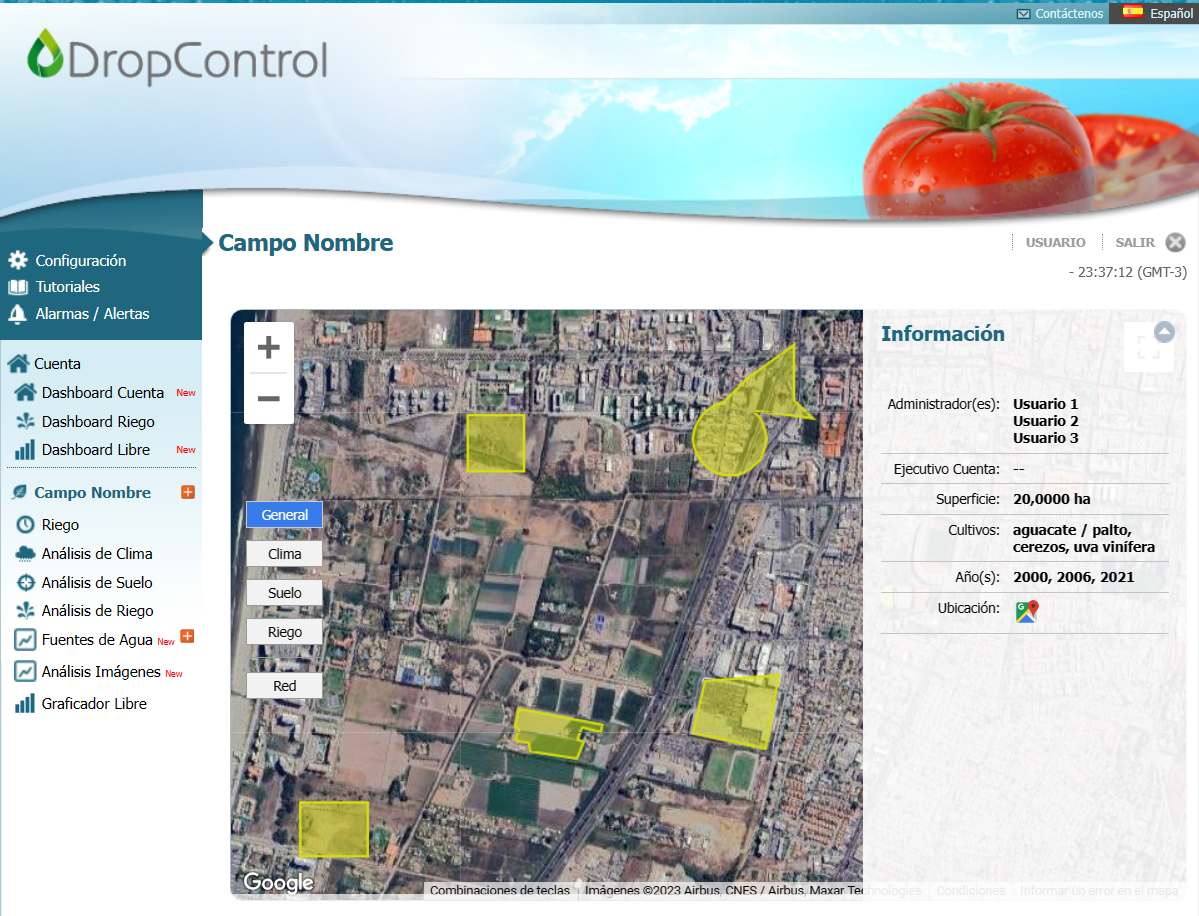
\includegraphics[width=0.8\textwidth]{mapa-dropcontrol}
	\caption{\label{fig:mapa-dropcontrol} \textit{Dashboard} de Campo - DropControl}
\end{figure}

Para mostrar el mapa se utiliza la api de \textit{Google Maps} y se utilizan los polígonos para marcar los sectores del campo y los marcadores para los nodos.
Para poder configurar este mapa existen dos maneras:
\begin{enumerate}
    \item En la aplicación \textit{Admin de DropControl}, ingresar de manera individual a cada sector/nodo y agregar su respectivo polígono/marcador de manera individual.
    \item Enviar un ticket al área de soporte con un archivo con formato \textit{.kmz} o \textit{.kml} que contiene los polígonos y/o marcadores para sus respectivos sectores y/o nodos.
\end{enumerate}
Para la primera opción, si el campo tiene demasiados sectores/nodos conllevará mucho tiempo en asignar los polígonos/marcadores respectivos.
En la segunda opción existen problemas como el tiempo que demora el área de soporte en tomar el ticket y realizar la configuración y/o
que las instrucciones no estén bien indicadas, llevando a que esta configuración requiera varios tickets para que se haga lo que el; cliente usuario necesita.

Es por esto que se plantea una herramienta en la aplicación de \textit{Admin de DropControl} para que el usuario cliente sea el que
configure el mapa, subiendo su archivo \textit{.kmz} o \textit{.kml} y asignando los polígonos/marcadores a sus respectivos sectores/nodos.
Junto con esto, también se agrega la funcionalidad de descargar el mapa de su campo en formato \textit{.kmz}.

¿Por qué usar formato \textit{.kmz}/\textit{.kml}? \textit{KML} (\textit{Keyhole Markup Language}) es un formato de archivo basado en \textit{XML} que se utiliza para mostrar datos geográficos en navegadores basados en la tierra, como \textit{Google Earth}. Un archivo \textit{KMZ}\footnote{\href{https://developers.google.com/kml/documentation/kmzarchives?hl=es-419}{Archivos KMZ}} está formado por un archivo \textit{KML} (doc.kml) y otros archivos comprimidos en un archivo zip.

En la figura \ref{fig:ejemplo_kml} se puede apreciar un ejemplo básico de un archivo \textit{KML}. Los polígonos estan en el tag \texttt{<Polygon>}, mientras que los marcadores están en el tag \texttt{<Point>}.
\begin{figure}[H]
    \centering
    \begin{lstlisting}[language=XML, frame=single]
        <?xml version="1.0" encoding="UTF-8"?>
        <kml>
        <Document>
            <name>Test file</name>                        
            <Placemark>
                <name>Polígono</name>
                <styleUrl>#s1</styleUrl>
                <Polygon>
                    <outerBoundaryIs>
                        <LinearRing>
                            <coordinates>
                                -119.4543294743033,
                                35.75022332932038,
                                0 -119.4501211374852,
                                35.75018426465995,
                                0 -119.4500004479587
                            </coordinates>
                        </LinearRing>
                    </outerBoundaryIs>
                </Polygon>
            </Placemark>            
            <Placemark>
                <name>Marcador</name>
                <Point>
                    <coordinates>
                        -119.445217337381,
                        35.75365570663719,
                        0
                    </coordinates>
                </Point>
            </Placemark>            
        </Document>
        </kml>        
    \end{lstlisting}
    \caption{Ejemplo de estructura KML para una librería. Fuente: Elaboración propia.}
    \label{fig:ejemplo_kml}
\end{figure}


Esta nueva herramienta se encontrará en la vista del campo; en el mapa del campo se encontrarán dos botones (en la posición que muestra la figura \ref{fig:mapcfg-farm}): Un botón para la descarga del mapa en formato \textit{.kmz} y, otro botón, para poder entrar al configurador de mapa.

\begin{figure}[H]
	\centering
	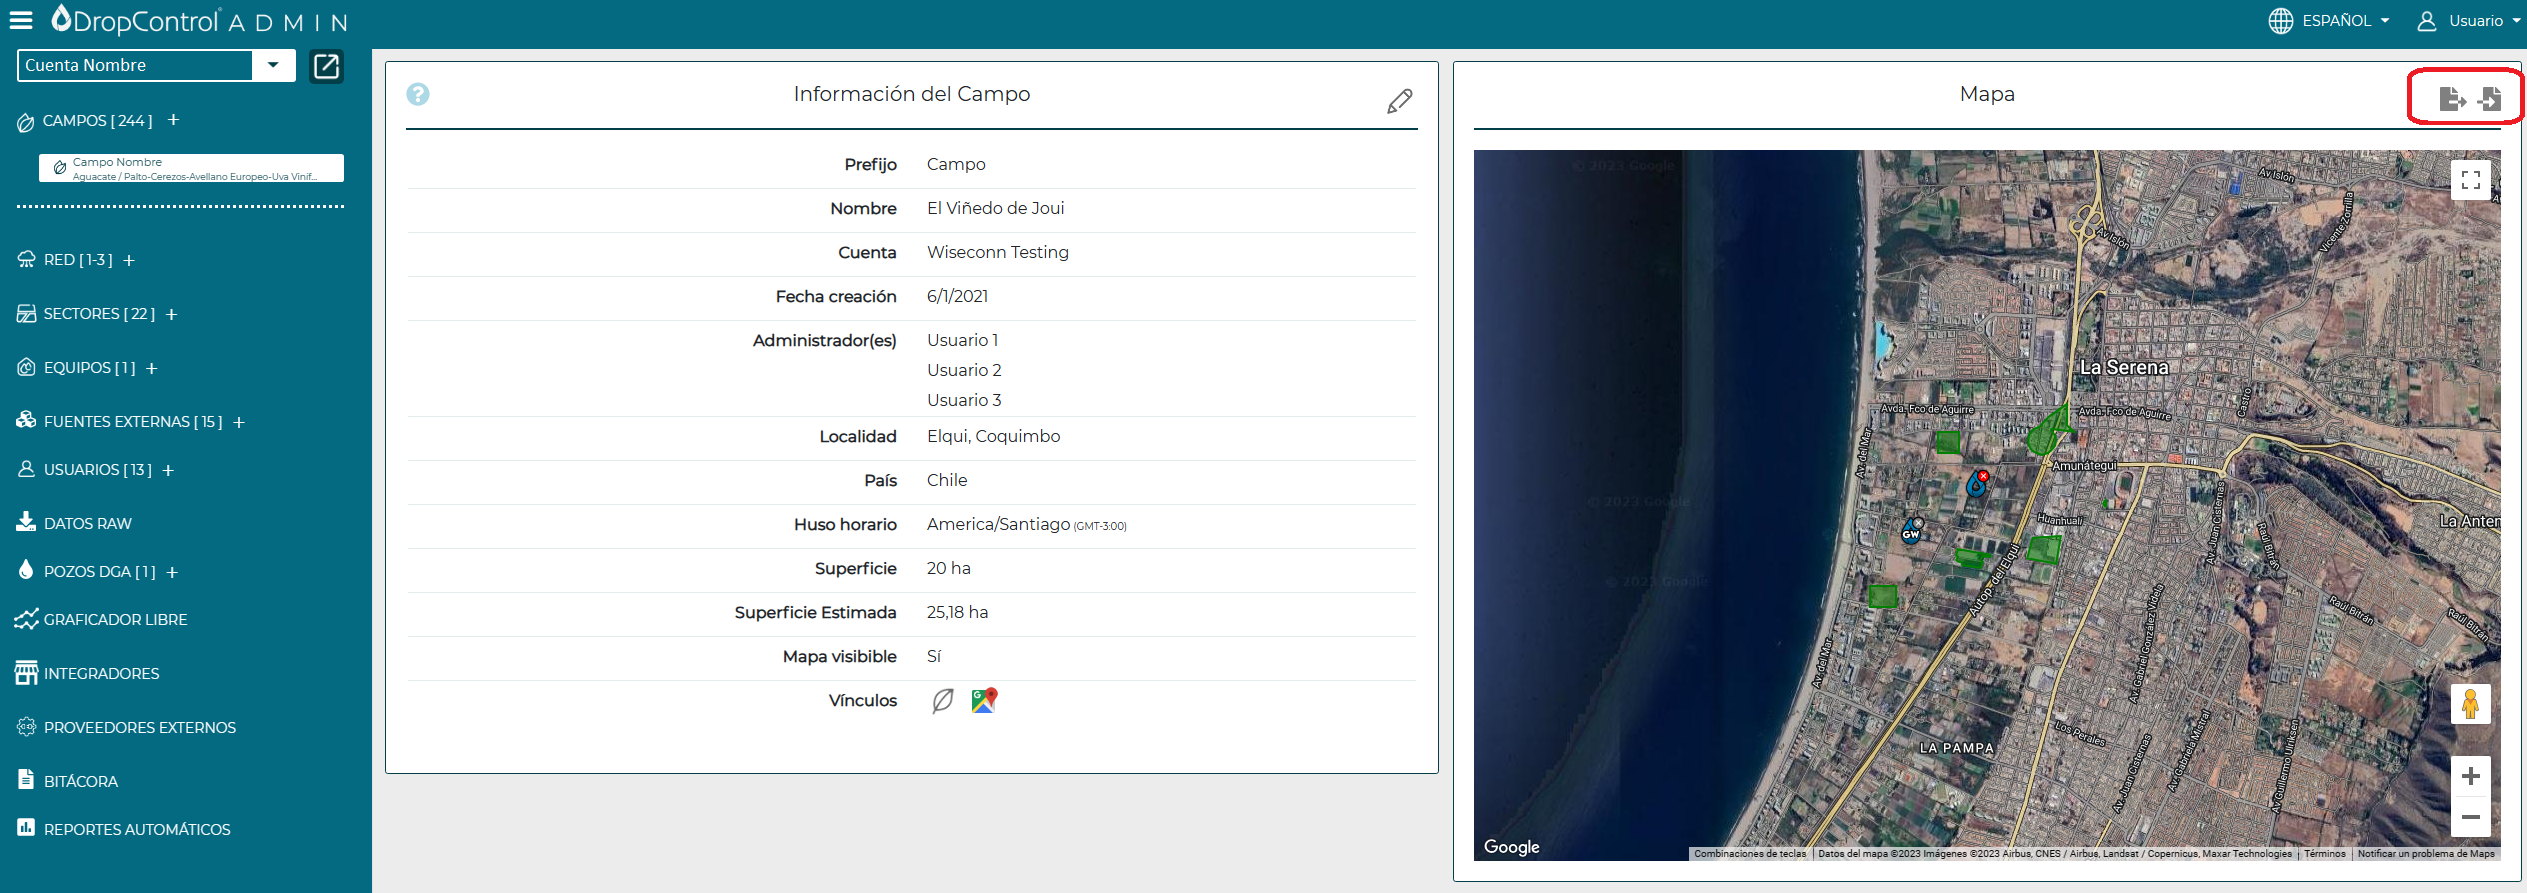
\includegraphics[width=0.8\textwidth]{mapcfg-farm}
	\caption{\label{fig:mapcfg-farm} Posición de botones de descarga de mapa y configurador de mapa.}
\end{figure}

Al hacer click en el botón de descarga del mapa, se descargará, valga la redundancia, el mapa del campo en un archivo con formato \textit{.kml}. El usuario podrá hacer cambios en ese archivo con aplicaciones que permitan la extensión \textit{.kml} (ejemplo, Google Earth) y después cargarlo en el configurador de mapa y actualizar sus sectores y/o nodos en el mapa del campo.

Al entrar en el configurador de mapa, esta vista se divide en 2 secciones (figura \ref{fig:mapcfg-esquema}): Tabla de sectores/nodos y el mapa.
\begin{figure}[H]
	\centering
	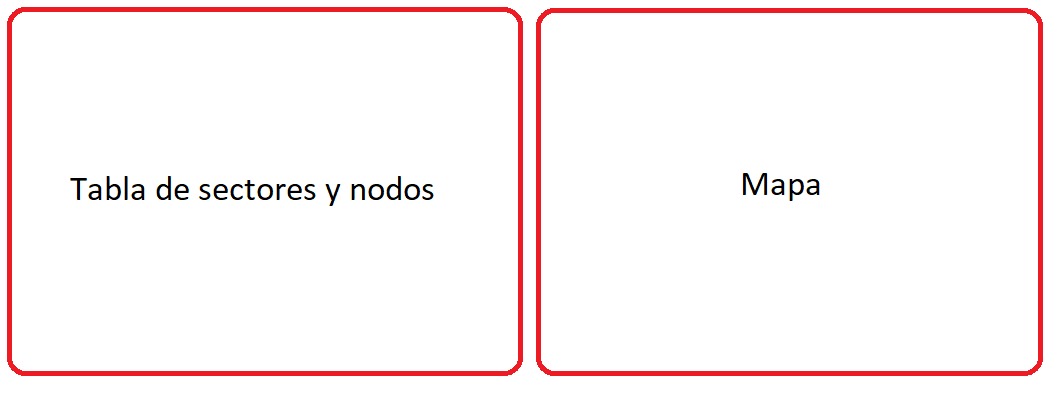
\includegraphics[width=0.8\textwidth]{mapcfg-esquema}
	\caption{\label{fig:mapcfg-esquema} Esquema de configurador de mapa. Fuente: Elaboración propia.}
\end{figure}

En la tabla de sectores/nodos (figura \ref{fig:mapcfg-tables-exameple}) se compone de:

\begin{itemize}
    \item \textbf{Botones:}
          \begin{itemize}
              \item En la parte superior izquierda están los botones para cambiar entre la tabla de sectores y nodos.
              \item En el lado opuesto, se encuentra el botón de 'Cargar Archivo' que, como indica el nombre, es para poder subir el archivo \textit{.kmz} o \textit{.kml} que contiene los polígonos y marcadores para asignar.
          \end{itemize}
    \item \textbf{Tabla:}  
    \begin{itemize}
        \item La tabla muestra los sectores o nodos, según lo seleccionado.
        \item En primera instancia contiene dos columnas, la primera con el nombre del sector/nodo y, la segunda es una columnna de acciones, con un botón que sirve para centrar el sector/nodo en el mapa. 
        \item Además, la tabla es paginada permitiendo al usuario elegir cuántos elementos mostrar por página.
    \end{itemize}
\end{itemize}

\begin{figure}[H]
	\centering
	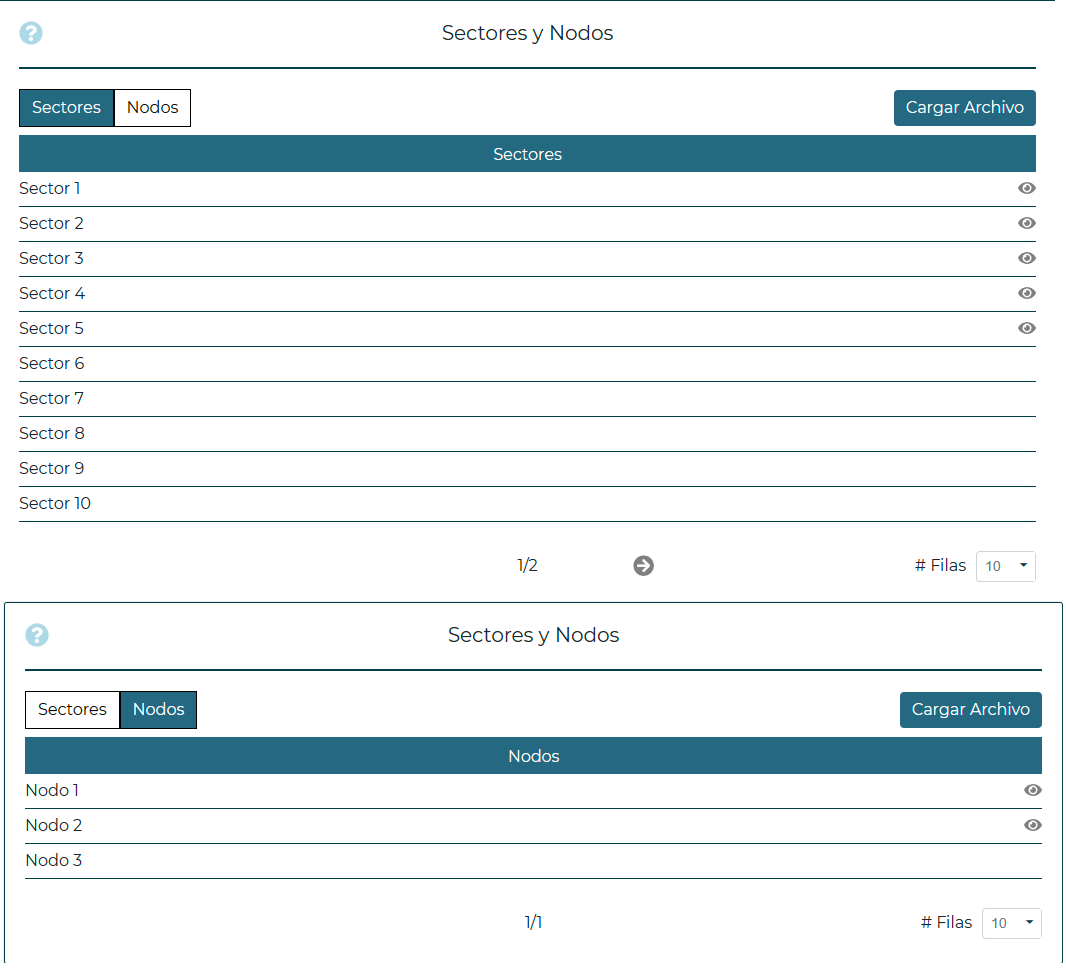
\includegraphics[width=0.8\textwidth]{mapcfg-tables}
	\caption{\label{fig:mapcfg-tables-exameple} Ejemplo tabla de sectores y nodos. Fuente: Elaboración propia.}
\end{figure}


Respecto al mapa, este muestra los sectores y/o nodos que estaban previamente asignados, los sectores los muestra con un color verde (figura \ref{fig:mapcfg-zone-pre}), mientras que los nodos los muestra con su ícono respectivo. Si está seleccionada la tabla de sectores en el mapa se muestran solo los polígonos, mismo caso con la tabla de nodos.
\begin{figure}[H]
	\centering
	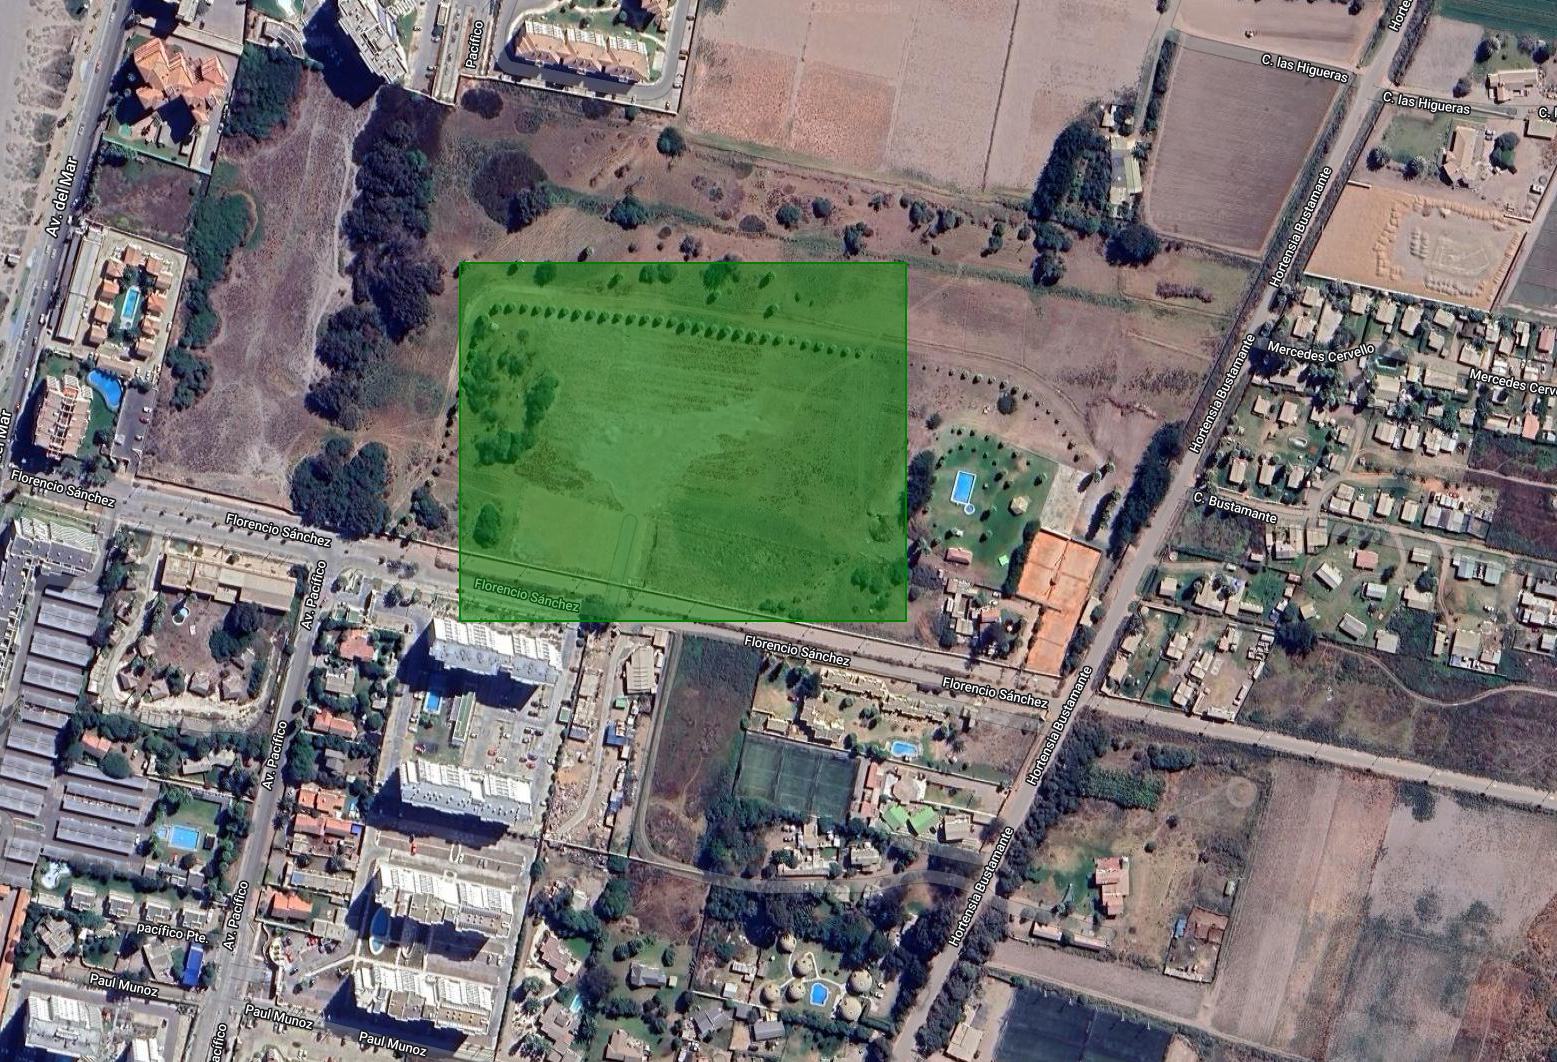
\includegraphics[width=0.8\textwidth]{mapcfg-zone-pre}
	\caption{\label{fig:mapcfg-zone-pre} Sector previamente asignado en el mapa}
\end{figure}

Al cargar un archivo, las secciones cambian. En la tabla de sectores/nodos ocurre lo siguiente (figura \ref{fig:mapcfg-tables-edit-exameple}):

\begin{itemize}
    \item El botón de 'Cargar Archivo' desaparece y se reemplaza por el nombre del archivo cargado junto a un ícono de basura que al hacerle click, elimina el archivo y vuelve al estado anterior.
    \item En la tabla ocurre lo siguiente:
    \begin{itemize}
        \item Se agrega una columna nueva al medio, que contiene un dropdown con los polígonos o nodos (según la tabla seleccionada) del archivo que se cargó recientemente (figura \ref{fig:mapcfg-add-zone-full}).
        \item En la columna de acciones:
        \begin{itemize}        
            \item Cuando un sector/nodo tiene un polígono/marcador previamente asignado, tiene las acciones de centrar en el mapa y descartar polígono/marcador.
            \item Al descartar un polígono/marcador previamente asignado, el botón de descartar se reemplaza por el botón de volver a polígono/marcador original.
            \item Para sectores/nodos que tengan asignados polígonos/marcadores, tienen disponible el botón para centrar en el mapa.
        \end{itemize}
    \end{itemize}
    \item En el mapa se agregan los polígonos/marcadores del archivo cargado previamente. Para los polígonos se muestran como en la figura \ref{fig:mapcfg-zone-loaded}, mientras que los nodos como en la figura \ref{fig:mapcfg-node-loaded}.
    \item Por último, debajo de la tabla se muestra el botón para guardar los cambios hechos en el mapa, al hacer click sobre este se abrirá un diálogo de confirmación que al ser aceptado, se guardarán los cambios y la herramienta volverá al estado en que no había un archivo cargado.
\end{itemize}

\begin{figure}[H]
	\centering
	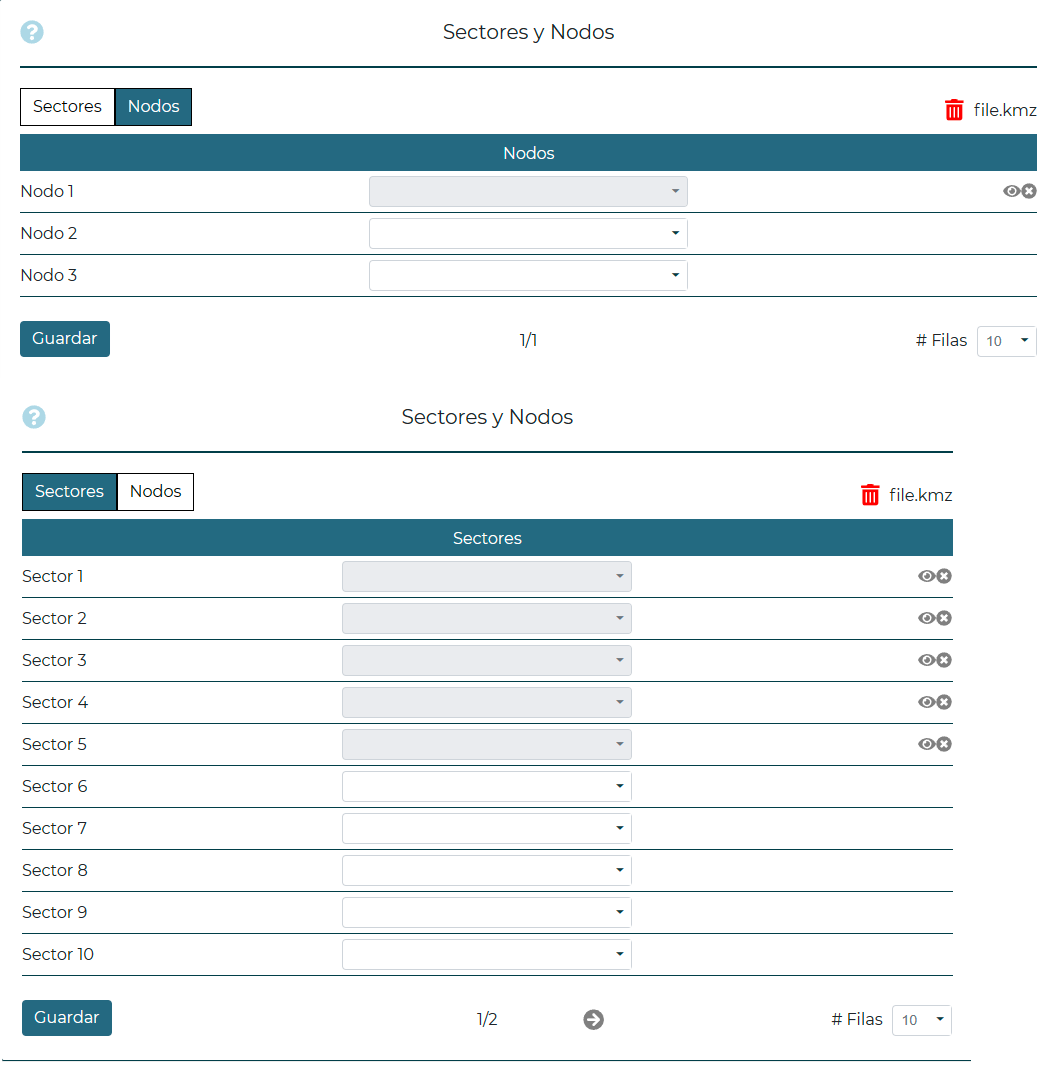
\includegraphics[width=0.8\textwidth]{mapcfg-tables-edit}
	\caption{\label{fig:mapcfg-tables-edit-exameple} Ejemplo tabla de sectores y nodos al cargar un archivo. Fuente: Elaboración propia.}
\end{figure}

\begin{figure}[H]
	\centering
	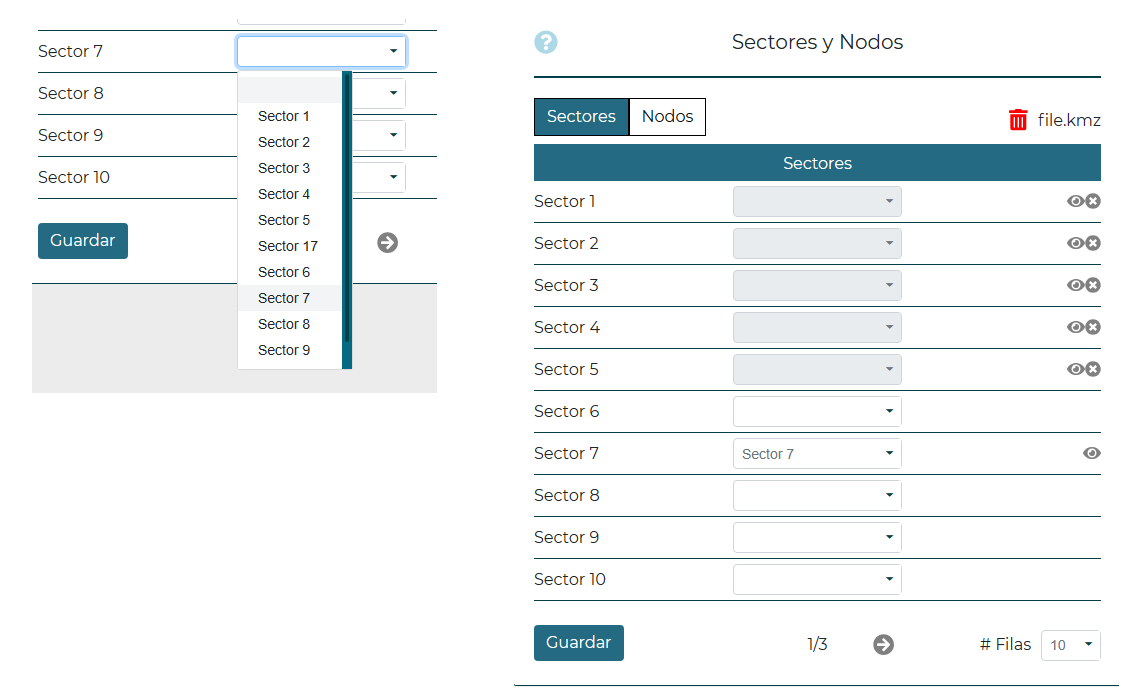
\includegraphics[width=0.8\textwidth]{mapcfg-add-zone-full}
	\caption{\label{fig:mapcfg-add-zone-full} Asignar un polígono a un sector. Fuente: Elaboración propia.}
\end{figure}

\begin{figure}[H]
	\centering
	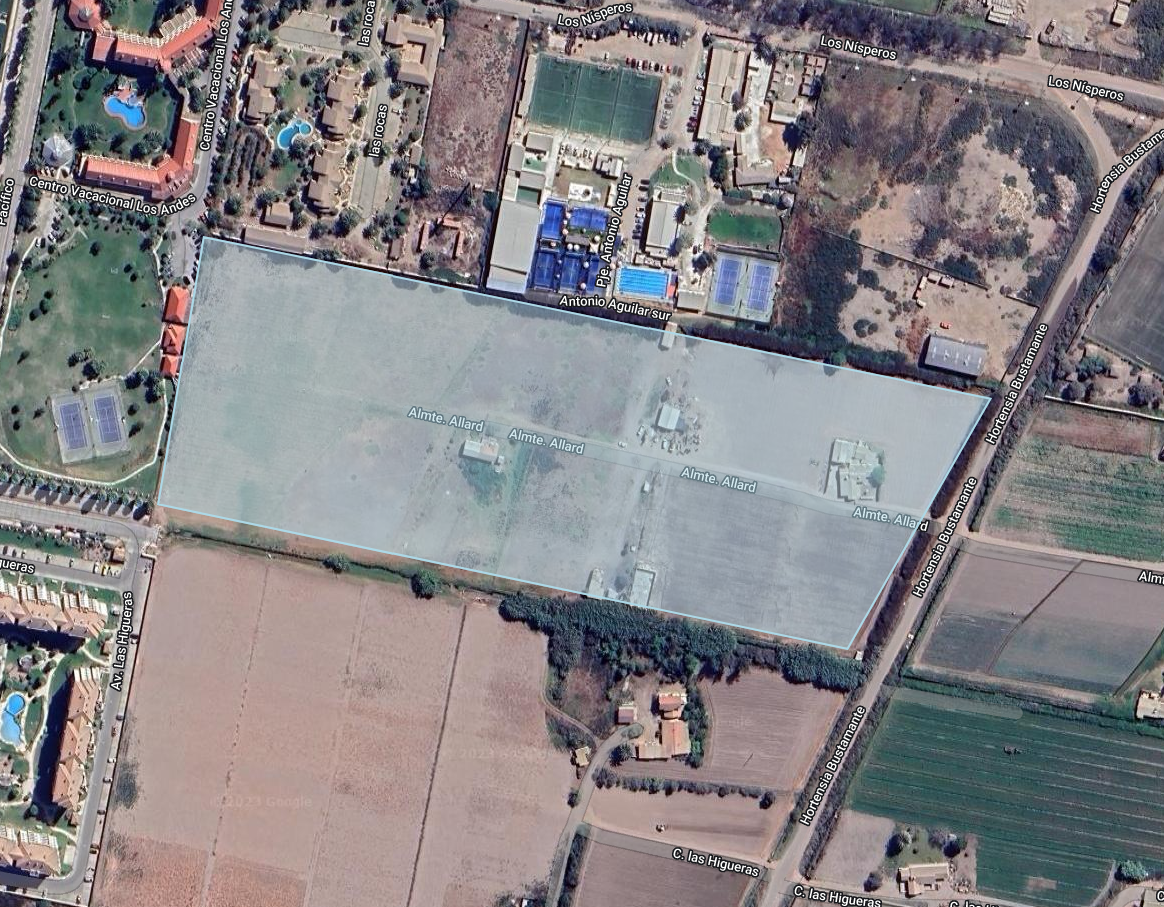
\includegraphics[width=0.8\textwidth]{mapcfg-zone-loaded}
	\caption{\label{fig:mapcfg-zone-loaded} Polígono cargado en el mapa}
\end{figure}

\begin{figure}[H]
	\centering
	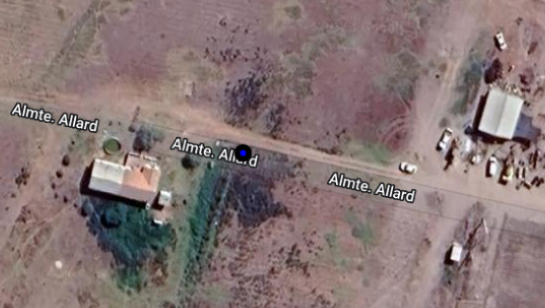
\includegraphics[width=0.8\textwidth]{mapcfg-node-loaded}
	\caption{\label{fig:mapcfg-node-loaded} Marcador cargado en el mapa}
\end{figure}

Para la acción de centrar un sector/nodo en el mapa, los polígonos/marcadores se verán de la siguiente forma:
\begin{itemize}
    \item Sector previamente asignado (figura \ref{fig:mapcfg-zone-pre-center}).
    \item Nodo previamente asignado (figura \ref{fig:mapcfg-node-pre-center}).
    \item Polígono cargado (figura \ref{fig:mapcfg-zone-loaded-center}).
    \item Marcador cargado (figura \ref{fig:mapcfg-node-loaded-center}).
\end{itemize}

\begin{figure}[H]
	\centering
	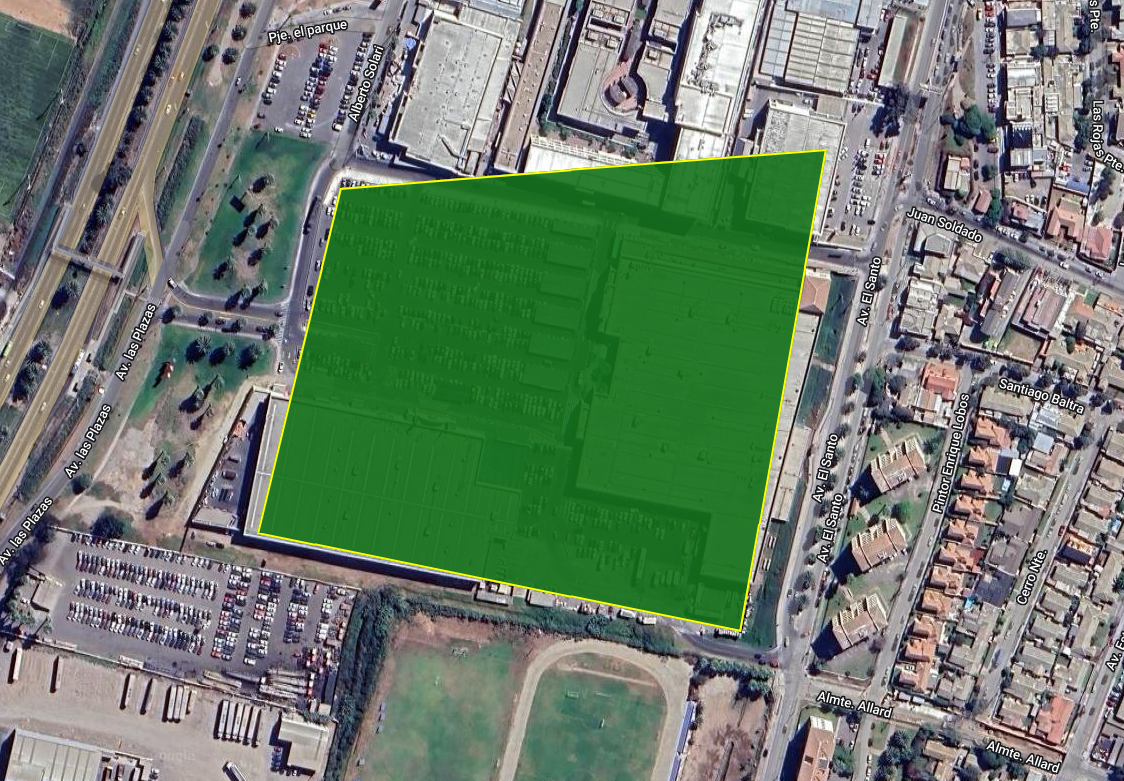
\includegraphics[width=0.8\textwidth]{mapcfg-zone-pre-center}
	\caption{\label{fig:mapcfg-zone-pre-center} Sector previamente asignado centrado en el mapa}
\end{figure}

\begin{figure}[H]
	\centering
	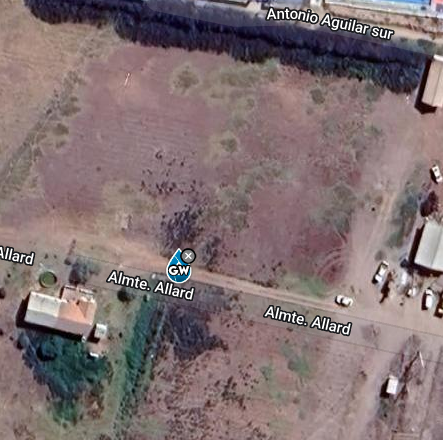
\includegraphics[width=0.8\textwidth]{mapcfg-node-pre-center}
	\caption{\label{fig:mapcfg-node-pre-center} Nodo previamente asignado centrado en el mapa}
\end{figure}

\begin{figure}[H]
	\centering
	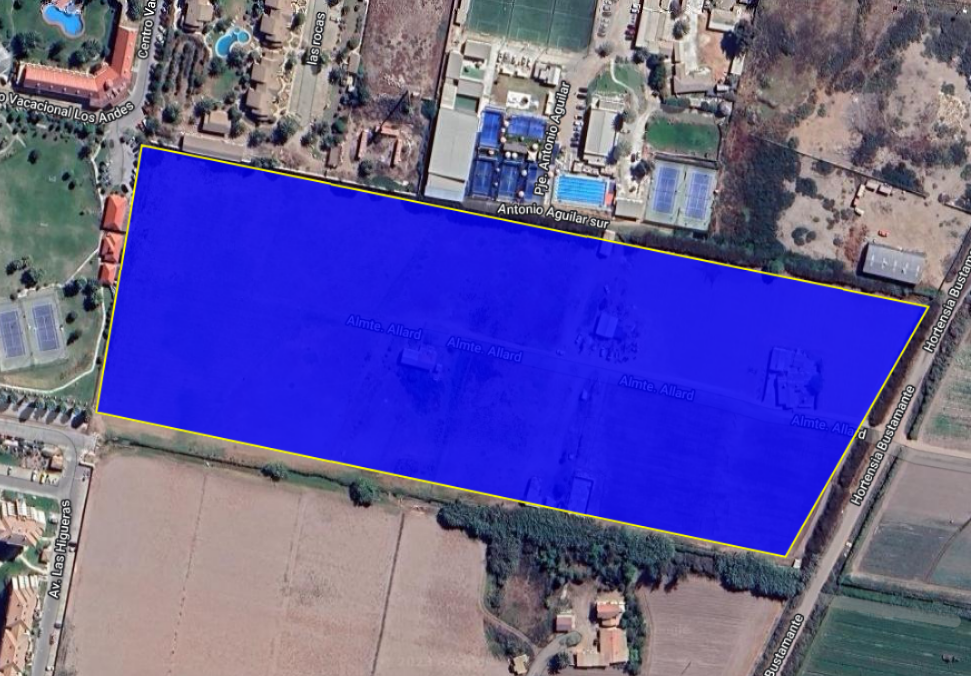
\includegraphics[width=0.8\textwidth]{mapcfg-zone-loaded-center}
	\caption{\label{fig:mapcfg-zone-loaded-center} Polígono cargado centrado en el mapa}
\end{figure}

\begin{figure}[H]
	\centering
	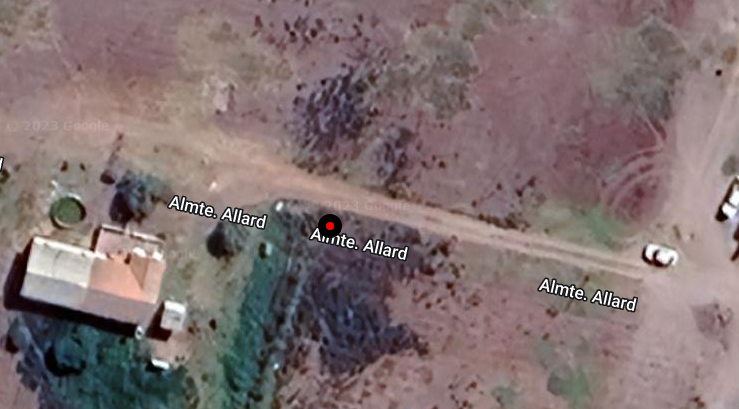
\includegraphics[width=0.8\textwidth]{mapcfg-node-loaded-center}
	\caption{\label{fig:mapcfg-node-loaded-center} Marcador cargado centrado en el mapa}
\end{figure}

Para finalizar, al hacer click en el botón 'Guardar', se abrirá un diálogo de confirmación para confirmar, valga la redundancia, los cambios hechos y guardarlos.
\iffalse
\subsubsubsection{GRAFICADOR LIBRE}

Como se explicó anteriormente, el plan gratuito que ofrece \textit{Wiseconn} sirve como punto de entrada a las herramientas
de pago de \textit{DropControl}. Sin embargo, el plan gratuito ofrece muy pocas funcionalidades y/o herramientas
implicando poca retención de los usuarios y no se cumplen con las especificaciones comerciales.

Los usuarios clientes de plan de pago tienen a su disposición un graficador en la aplicación de \textit{DropControl} (figura \ref{fig:graf-drop-classic}), en el cual
se pueden graficar los datos enviados por los nodos en los campos, dentro de un rango de tiempo.
Caso contrario ocurre para los usuarios clientes de plan gratuito, los cuales no poseen esta herramienta y
no pueden visualizar los datos de sus nodos.

\begin{figure}[H]
	\centering
	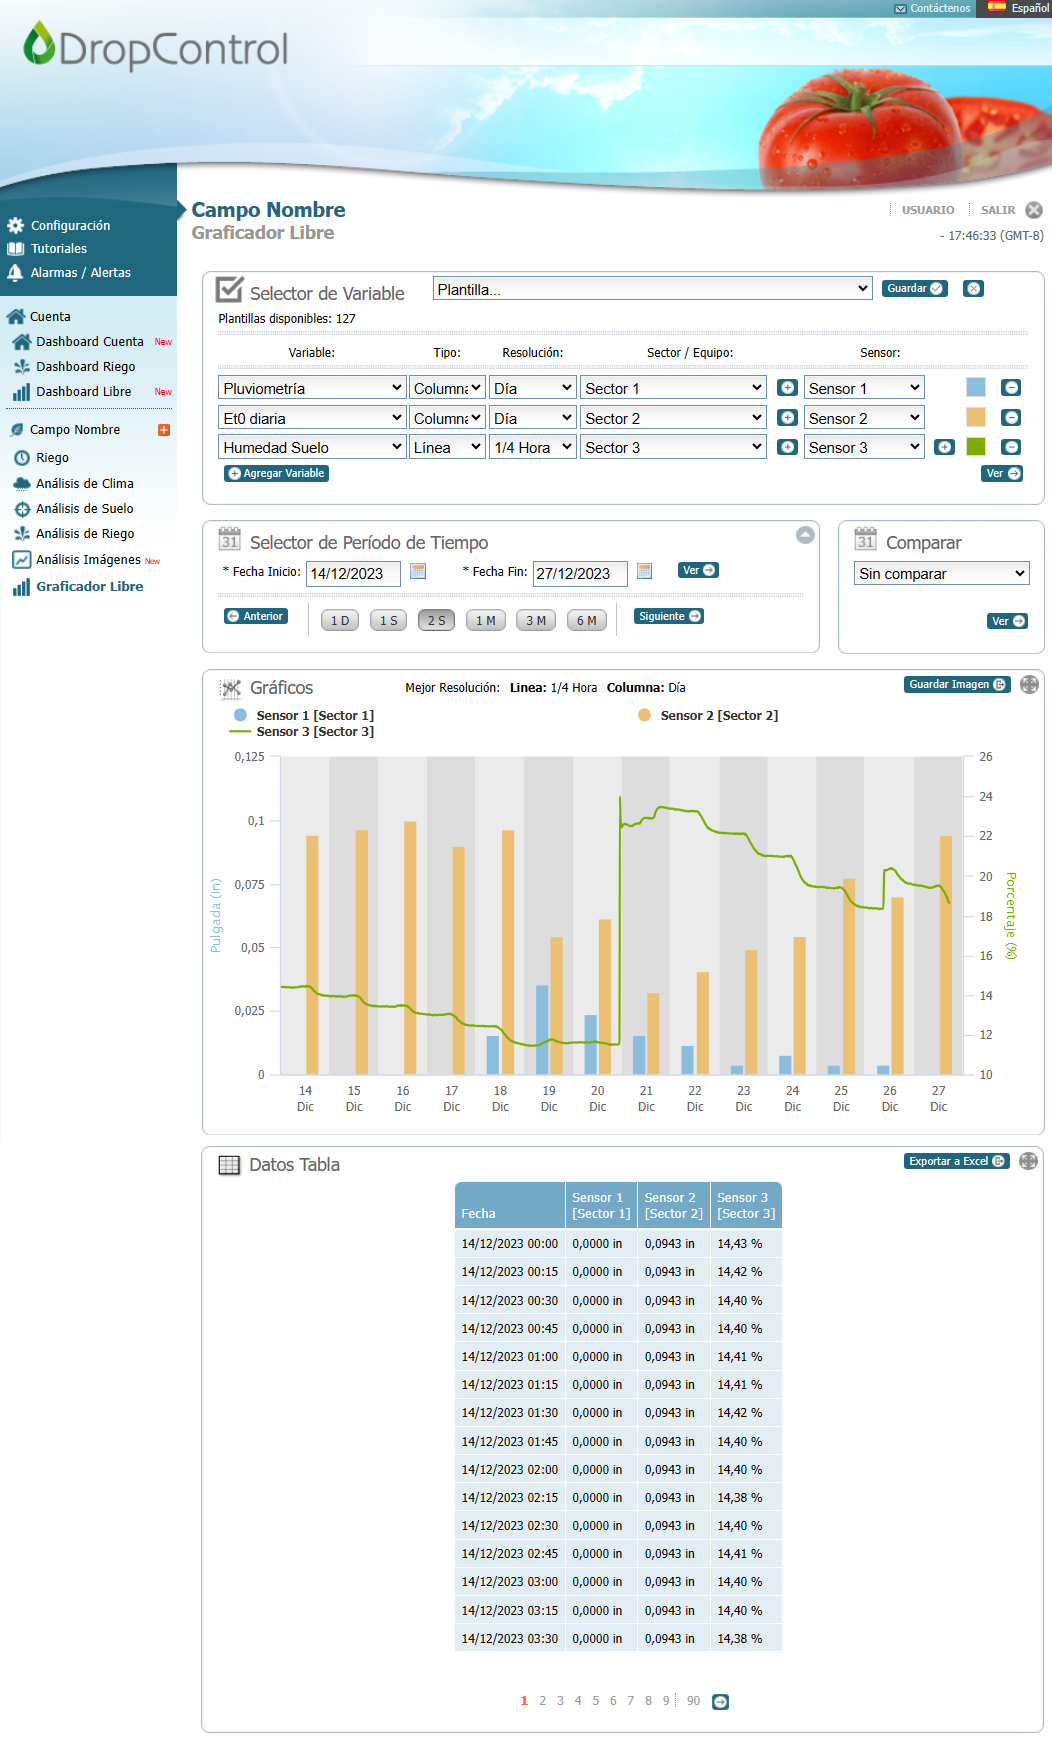
\includegraphics[width=0.5\textwidth]{graf-drop-classic}
	\caption{\label{fig:graf-drop-classic} Graficador Libre en \textit{DropControl}}
\end{figure}

Por esto se desarrolla la herramienta de 'Graficado Libre' en la aplicación de \textit{Admin de DropControl},
donde el usuario podrá escoger hasta 6 sensores para graficar en un rango de tiempo máximo de los últimos 3 meses (90 días).

Esta nueva herramienta se podrá acceder en el menú de \textit{Admin de DropControl} como muestra en la figura \ref{fig:menu-admin-graf1} bajo el nombre de `Graficador Libre`. 

\begin{figure}[H]
	\centering
	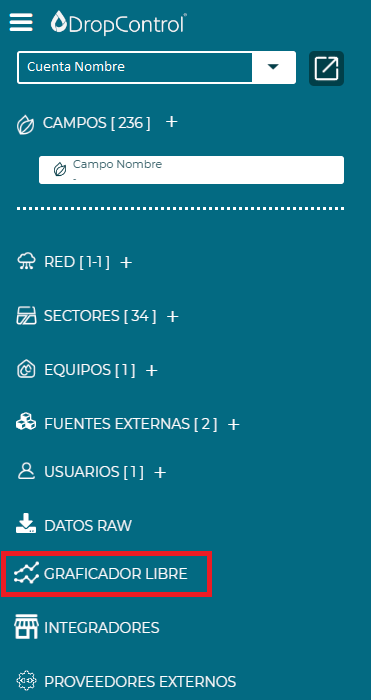
\includegraphics[width=0.5\textwidth]{menu-admin-graficador}
	\caption{\label{fig:menu-admin-graf1} Graficador Libre en el menú de \textit{Admin}}
\end{figure}

El graficador libre tendrá el esquema mostrado en la figura \ref*{fig:graf-esquema}

\begin{figure}[H]
	\centering
	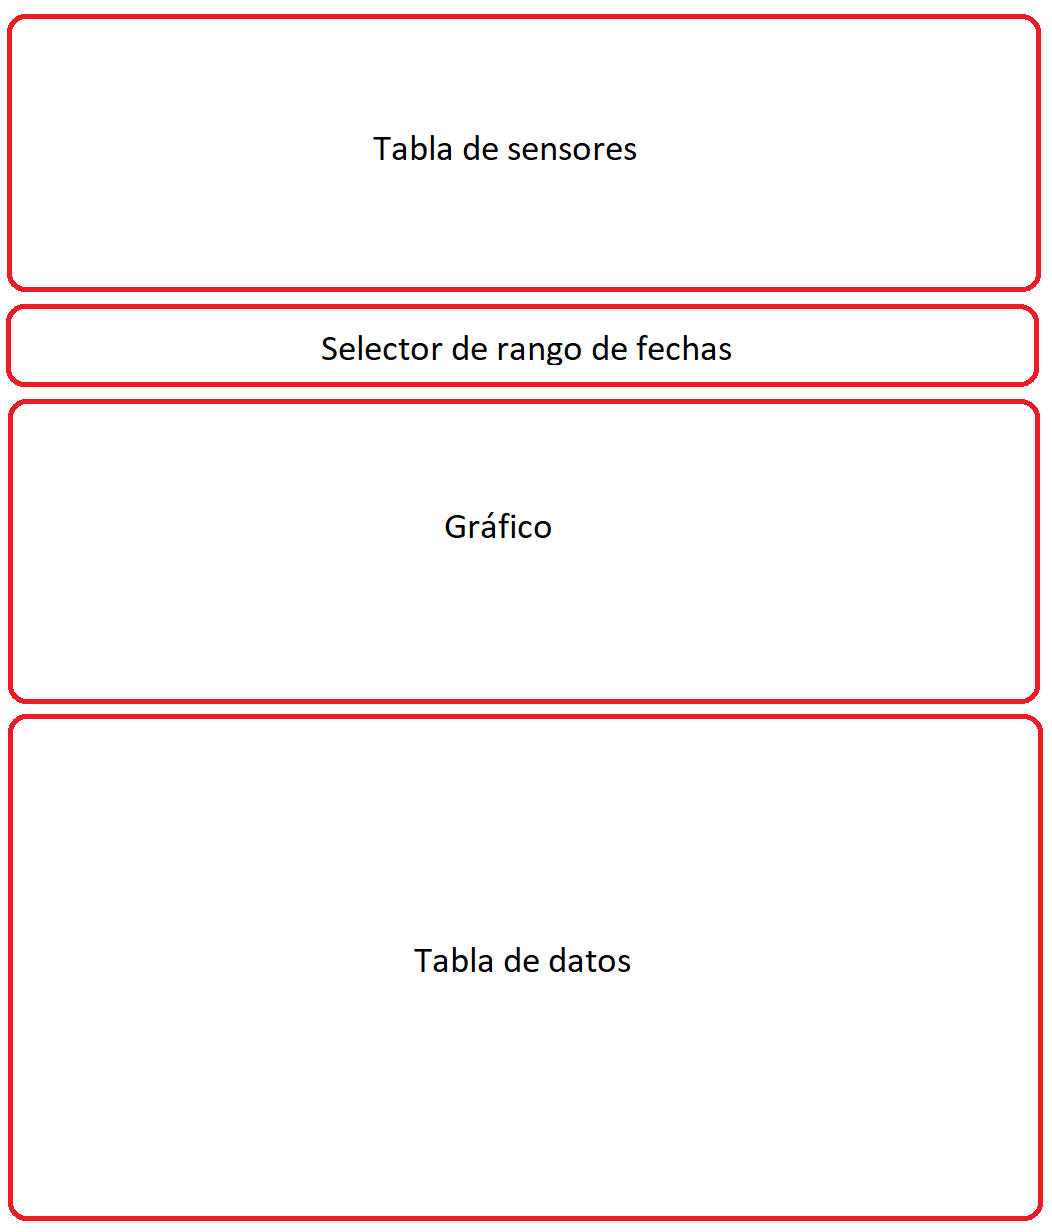
\includegraphics[width=0.5\textwidth]{graf-esquema}
	\caption{\label{fig:graf-esquema} Esquema graficador libre. Fuente: Elaboración propia.}
\end{figure}

En la tabla de sensores es donde se seleccionan los sensores que se quieren desplegar en el gráfico. Esta tabla tiene las siguientes propiedades y componentes (figura \ref{fig:graf-table}):
\begin{itemize}
    \item En primera instancia, la tabla empieza con una fila (figura \ref{fig:graf-table-empty}).
    \item Se podrá escoger hasta 6 sensores.
    \item Las columnas de la tabla son las siguientes:
          \begin{enumerate}
              \item Selector de nodos.
              \item Selector de sensores.
              \item Selector de color.
              \item Botón para eliminar fila (aparece cuando se tiene más de una fila).
          \end{enumerate}
    \item Botón para agregar una fila vacía.
\end{itemize}

\begin{figure}[H]
	\centering
	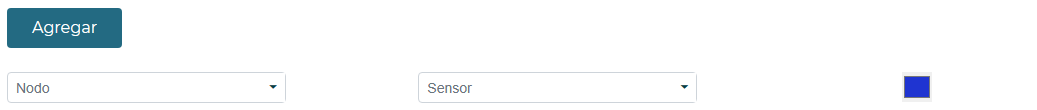
\includegraphics[width=0.8\textwidth]{graf-table-empty}
	\caption{\label{fig:graf-table-empty} Tabla de sensores vacía. Fuente: Elaboración propia.}
\end{figure}

\begin{figure}[H]
	\centering
	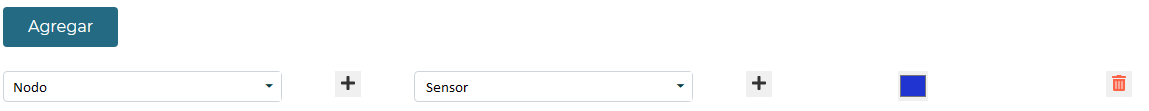
\includegraphics[width=0.8\textwidth]{graf-table}
	\caption{\label{fig:graf-table} Componentes de la tabla de sensores. Fuente: Elaboración propia.}
\end{figure}

Los sensores pertenecen a un nodo, es por esto que primero se debe seleccionar el nodo en el primer selector, para luego seleccionar el sensor perteneciente a ese nodo.
Para agregar nuevas filas a la tabla de sensores existen 3 formas.
\begin{enumerate}
    \item Haciendo click en el botón de `Agregar fila` que está en la esquina superior derecha de la tabla.
    \item Al escoger un nodo, al lado del selector aparecerá un botón con el signo `+` (figura \ref{fig:graf-table}). Al hacer click en ese botón agregará una nueva fila con el nodo siguiente en la lista seleccionado.
    \item Al escoger un sensor, al lado del selector aparecerá un botón con el signo `+` (figura \ref{fig:graf-table}). Al hacer click en ese botón agregará una nueva fila con el nodo seleccionado en la fila anterior, junto al sensor siguiente en la lista.
\end{enumerate}

En cuanto al selector de rango de fecha (figura \ref{fig:graf-chart-daterange-example}), se podrá escoger un máximo de los últimos 90 días. Además, existirán rangos predeterminados para que el usuario pueda escoger:
\begin{itemize}
    \item Últimos 7 días.
    \item Este mes.
    \item Últimos 30 días.
    \item Últimos 60 días.
    \item Últimos 90 días.
\end{itemize}
Para esto se utilizará el componente \textit{DateRangePicker} de \textit{Syncfusion}\footnote{\href{https://ej2.syncfusion.com/react/documentation/daterangepicker/getting-started}{Syncfusion: DateRangePicker}}.
\begin{figure}[H]
	\centering
	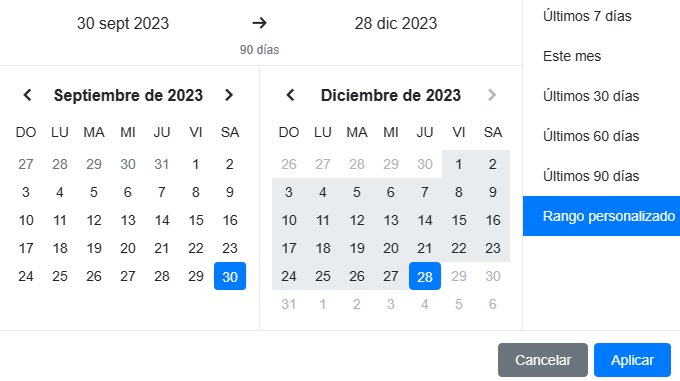
\includegraphics[width=0.8\textwidth]{graf-chart-daterange-example}
	\caption{\label{fig:graf-chart-daterange-example} Ejemplo de componente \textit{DateRangePicker}. Fuente: Elaboración propia.}
\end{figure}
Respecto al gráfico, se utilizará \textit{Highcharts Stock}\footnote{\href{https://www.highcharts.com/docs/stock/understanding-highcharts-stock}{Understanding Highcharts Stock}} para poder desplegar los datos. Cada serie del gráfico representa un sensor que se escogió en la tabla de sensores (figura \ref{fig:graf-chart-example}). La serie tendrá un formato de nombre [Nodo]-[Sensor].
\begin{figure}[H]
	\centering
	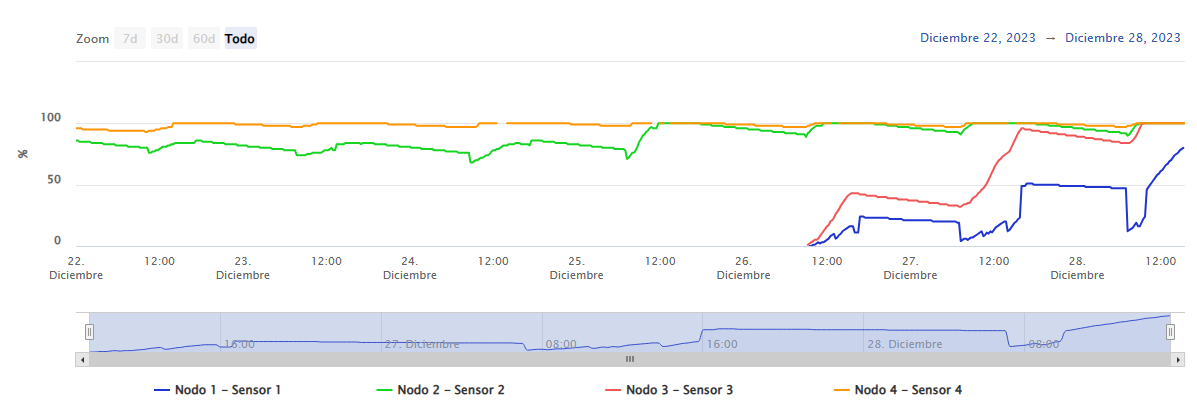
\includegraphics[width=0.8\textwidth]{graf-chart-example}
	\caption{\label{fig:graf-chart-example} Ejemplo de gráfico. Fuente: Elaboración propia.}
\end{figure}

Al pasar el puntero por encima de las series, se mostrará un \textit{tooltip} con el dato de las series (figura \ref{fig:graf-chart-tooltip}).
\begin{figure}[H]
	\centering
	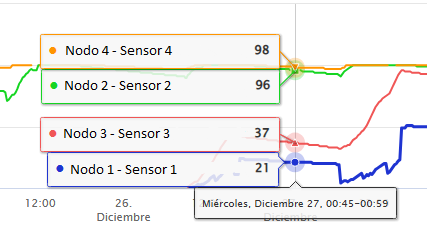
\includegraphics[width=0.5\textwidth]{graf-chart-tooltip}
	\caption{\label{fig:graf-chart-tooltip} \textit{Tooltip}. Fuente: Elaboración propia.}
\end{figure}
El estar usando \textit{Highcharts Stock}, nos permite realizar las siguientes acciones:
\begin{itemize}
    \item Se podrá hacer zoom, ya sea, de forma manual, seleccionado el rango en el gráfico o haciendo click en las opciones para ver rangos de 7, 30, 60 días en la esquina superior izquierda (dependiendo del rango de fechas seleccionado). También se podrá usar el \textit{navigator}\footnote{\href{https://www.highcharts.com/docs/stock/navigator}{Highcharts Stock Navigator}} que proporciona la biblioteca.
    \item Esconder/mostrar series del gráfico haciendo click en la leyenda de la serie.
\end{itemize}

Por último tenemos la tabla de datos del gráfico (figura \ref{fig:graf-chart-table-example}), para esto se utilizará el componente \textit{Grid}\textit{Syncfusion}\footnote{\href{https://ej2.syncfusion.com/react/documentation/grid/getting-started}{Syncfusion: Grid}} de \textit{Syncfusion}, que permite agregar la acción de \textit{Sorting} por columna y exportar la tabla en formato .xls.
La tabla tiene las siguientes propiedades:
\begin{itemize}
    \item La primera columna corresponde a la fecha y las columnas siguientes corresponden a las combinaciones de nodos/sensores seleccionados.
    \item La tabla es paginada y se puede cambiar el número de filas a mostrar por cada página.
    \item La tabla se ordena por fecha del dato, se puede cambiar el orden ascendente/descendente, haciendo click en el header de la columna.
    \item En la esquina superior derecha habrá un botón con el cual se podrá descargar la tabla en formato .xls.
\end{itemize}

\begin{figure}[H]
	\centering
	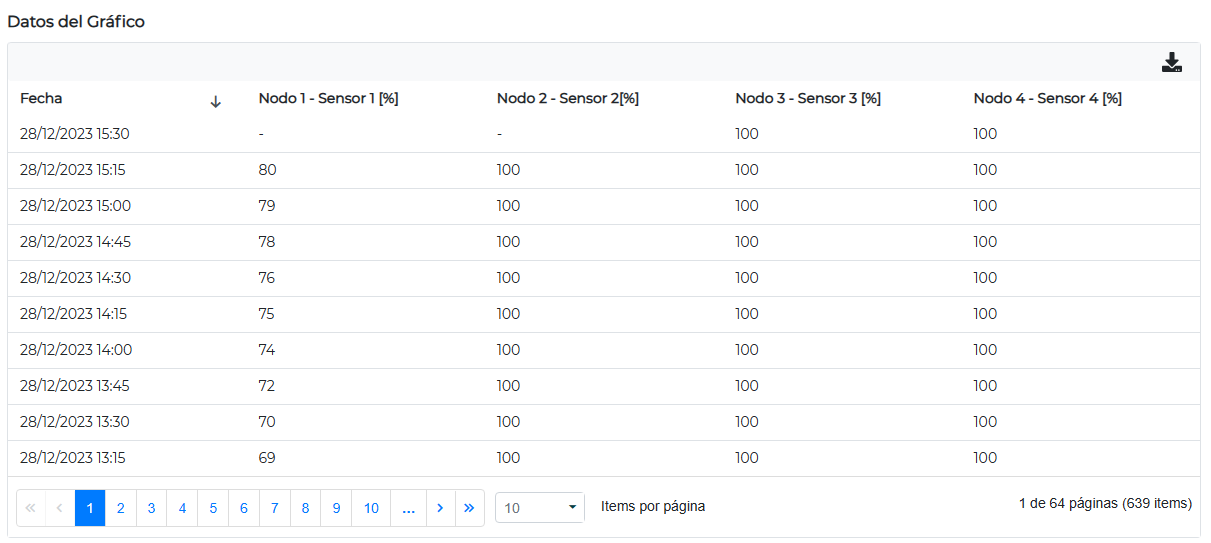
\includegraphics[width=0.8\textwidth]{graf-chart-table-example}
	\caption{\label{fig:graf-chart-table-example} Ejemplo de tabla de datos. Fuente: Elaboración propia.}
\end{figure}\fi

\subsubsection{OPERATIONS}

El área de producción se encarga del ensamblado y testeo del hardware de WiseConn, junto con el su inventario y despachos de estos. Para llevar registro de todo esto se utiliza la aplicación de \textit{Operations}

En \textit{Operations} se puede hacer:

\begin{itemize}
    \item Configurar los tipos de productos.
    \item Administrar lotes de productos.
    \item Administrar despachos de productos.
    \item Llevar el inventario de los productos y los estados de estos, gracias a que cada producto tiene asociado un historial.
\end{itemize}
\iffalse
\subsubsubsection{DESPACHOS MÚLTIPLES}

En \textit{Operations}, como se mencionó anteriormente, se administran los despachos de los distintos productos de hardware que ofrece \textit{WiseConn}.
La sección de despachos (figura \ref{fig:dm-mantenedor-indv}) se compone de una tabla que contiene los despachos existentes. La tabla contiene botónes de acciones de crear, editar, eliminar y exportar a CSV en el \textit{header} y \textit{footer} de este, además, en la parte izquierda del \textit{header} existe un filtro de rango de fecha. 
Para las acciones de ver, eliminar y cerrar es necesario primero seleccionar una fila de la tabla para que se habilite el botón.
De igual manera, existen filtros por columnas como se ve en la figura \ref{fig:dm-mantenedor-indv-filters}.

\begin{figure}[H]
	\centering
	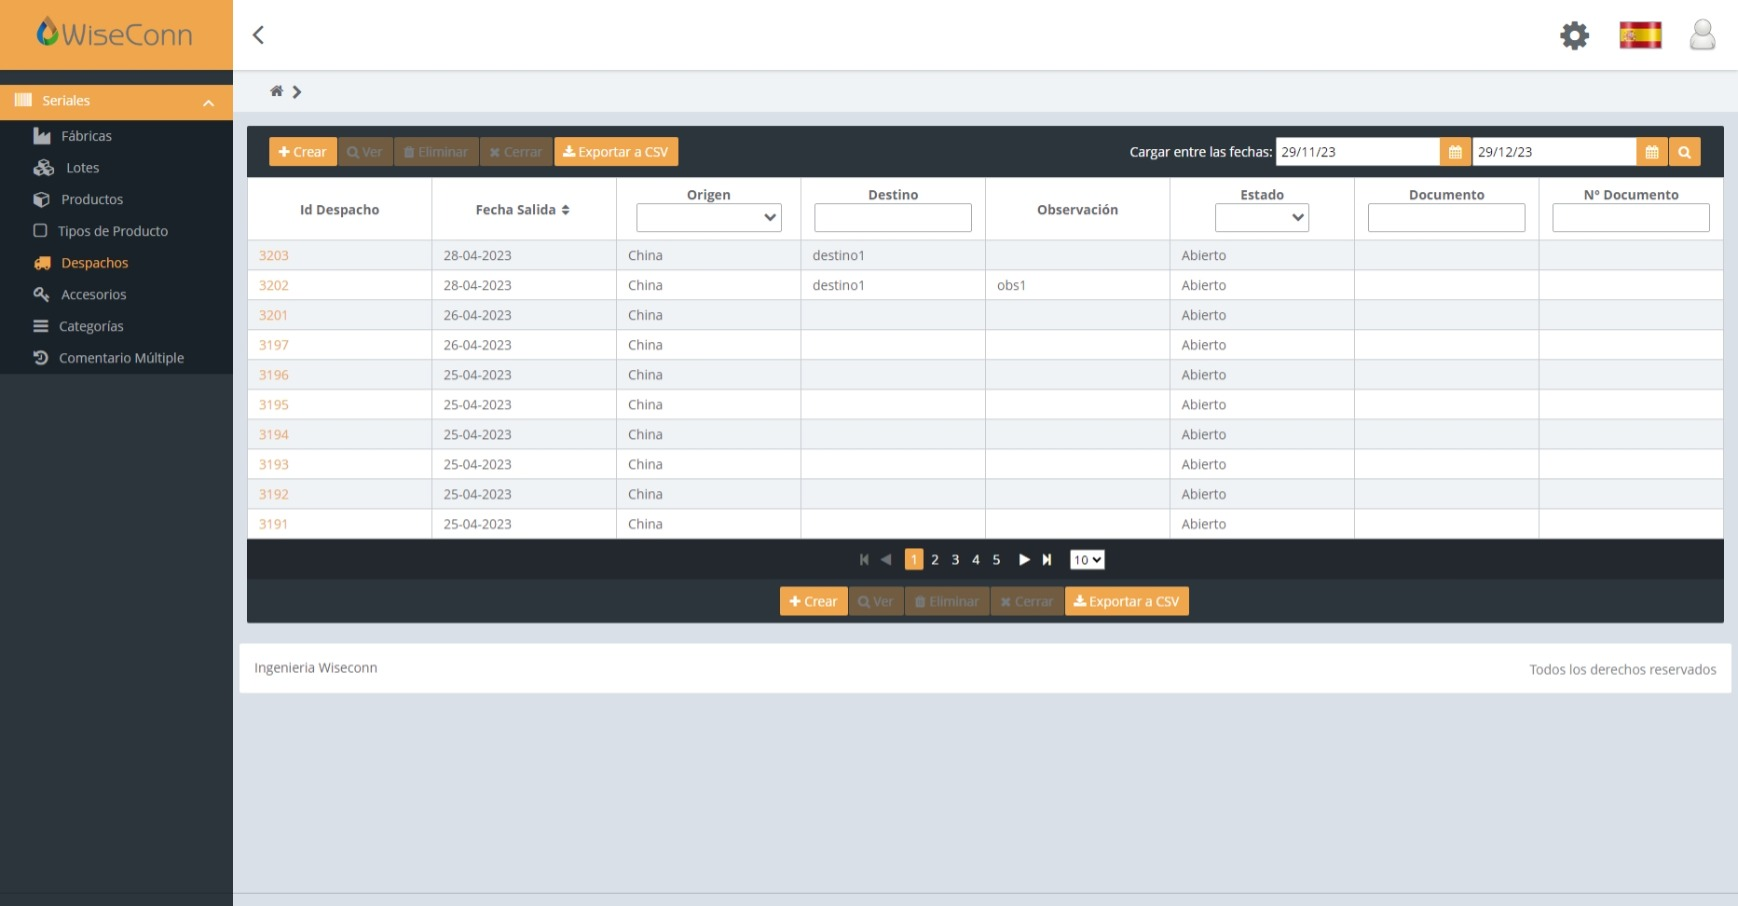
\includegraphics[width=0.8\textwidth]{dm-mantenedor-indv}
	\caption{\label{fig:dm-mantenedor-indv} Sección de despachos. Fuente: Elaboración propia.}
\end{figure}

\begin{figure}[H]
	\centering
	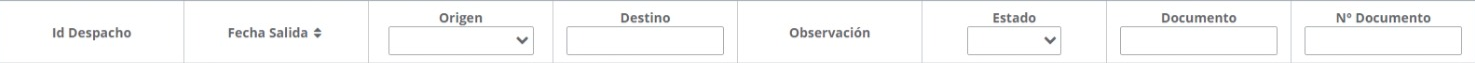
\includegraphics[width=0.8\textwidth]{dm-mantenedor-indv-filters}
	\caption{\label{fig:dm-mantenedor-indv-filters} Filtros por columna. Fuente: Elaboración propia.}
\end{figure}

Al hacer click en el botón crear, se abre un siguiente formulario (figura \ref{fig:dm-create-indv-form}) para ingresar las propiedades:
\begin{itemize}
    \item Fecha de salida
    \item Fecha de activación
    \item Destino
    \item País destino
    \item Observación
    \item Documento
    \item Número de documento
    \item Despacho interno \textit{flag}    
\end{itemize}

\begin{figure}[H]
	\centering
	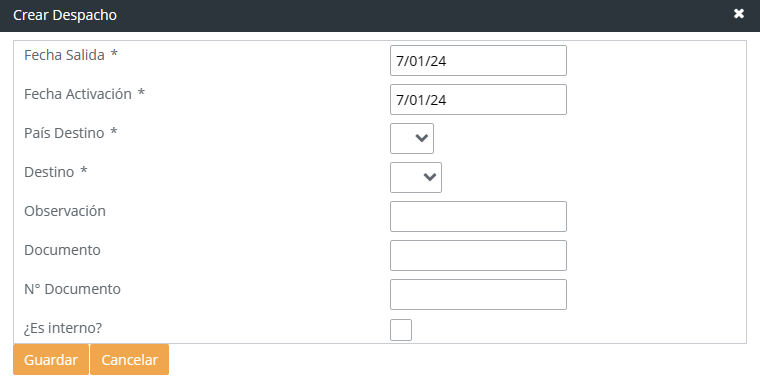
\includegraphics[width=0.5\textwidth]{dm-create-indv-form}
	\caption{\label{fig:dm-create-indv-form} Formulario creación de Despacho. Fuente: Elaboración propia.}
\end{figure}

Para poder entrar a un despacho se debe hacer click en la fila de la tabla y hacer click en el botón ver, al igual que haciendo click en la Id del despacho.
La vista del despacho se muestra en la figura \ref{fig:dm-vista-indv}.

\begin{figure}[H]
	\centering
	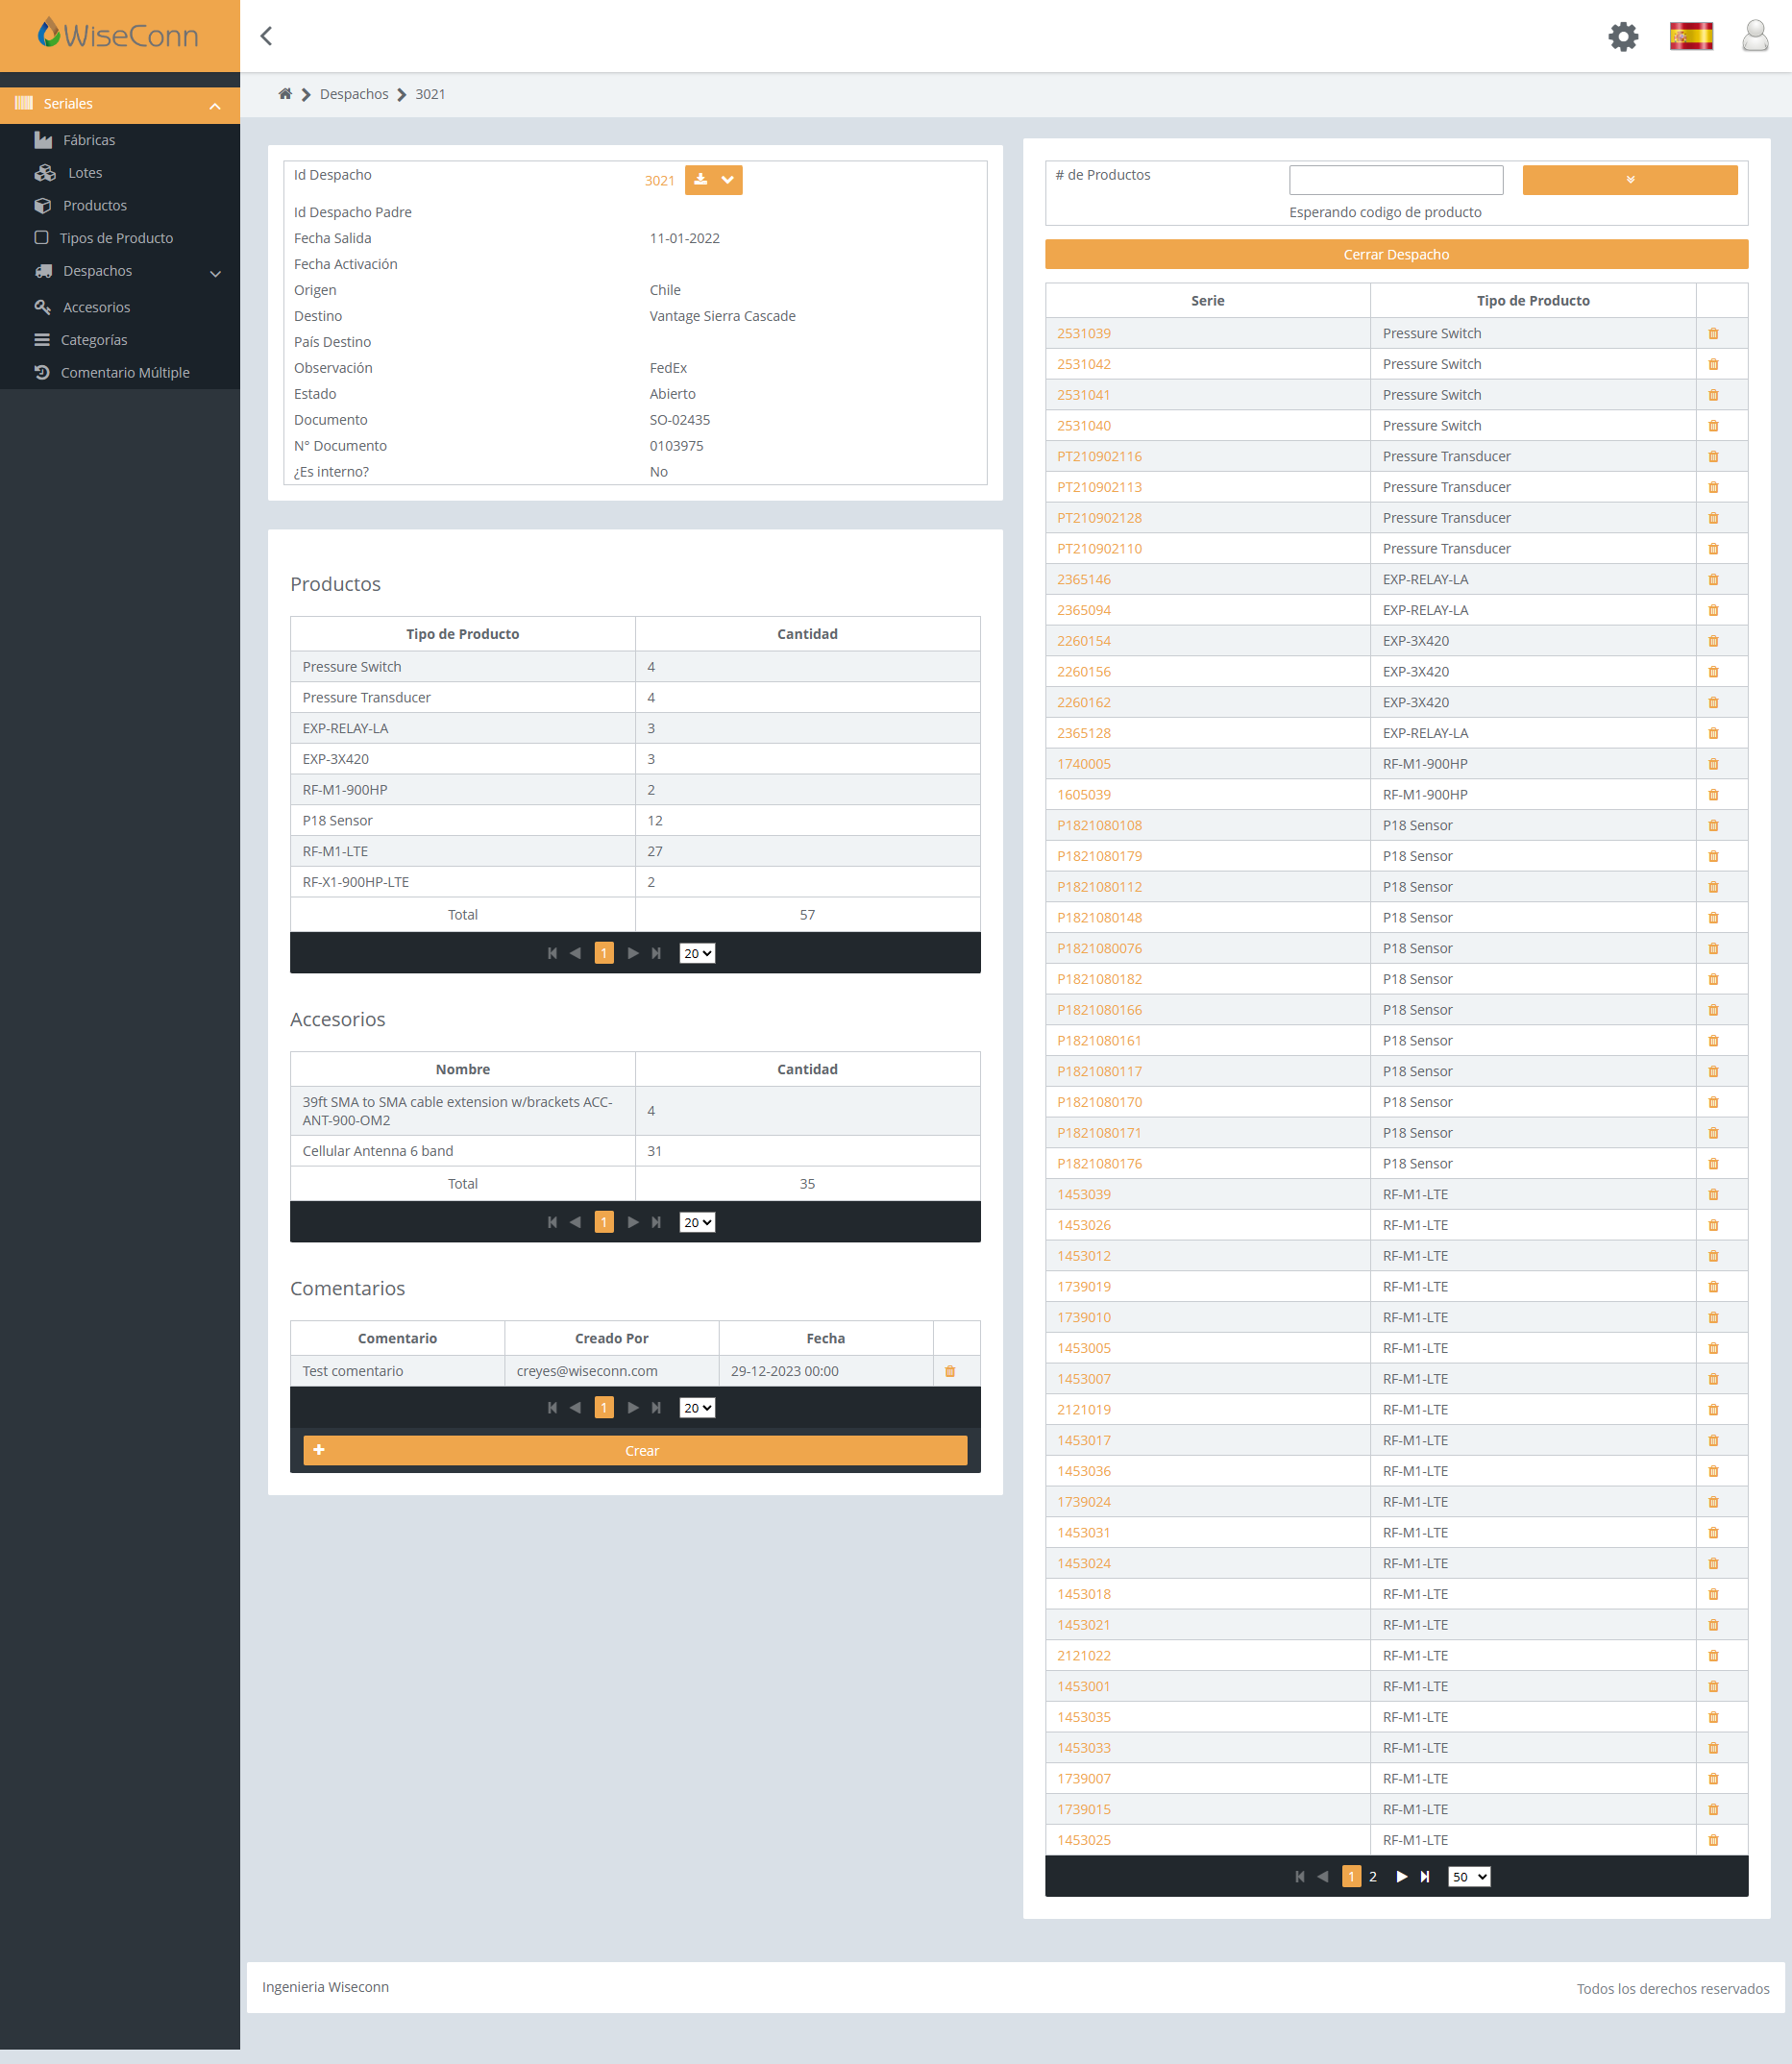
\includegraphics[width=0.8\textwidth]{dm-vista-indv}
	\caption{\label{fig:dm-vista-indv} Vista de despacho. Fuente: Elaboración propia.}
\end{figure}

La vista del despacho contiene las siguientes secciones:
\begin{itemize}
    \item En el lado derecho:
    \begin{itemize}
        \item \textit{Input} para ingresar la serie del producto o código de accesorio.
        \item Tabla de productos. Columnas: Series, tipo de producto, acción de eliminar.
    \end{itemize}
    \item En el lado izquierdo:
    \begin{itemize}
        \item Información del despacho.
        \item Resumen de productos.
        \item Resumen de accesorios.
        \item Tabla de comentarios.
    \end{itemize}
\end{itemize}

En la vista de un despacho se pueden editar las propiedades de este, como muestra en la figura \ref{fig:dm-indv-edit}, haciendo click sobre el dato se cambiará a un input correspondiente al tipo de dato (fecha, texto, select, etc.). También es posible agregar productos y accesorios y descargar un reporte.

\begin{figure}[H]
	\centering
	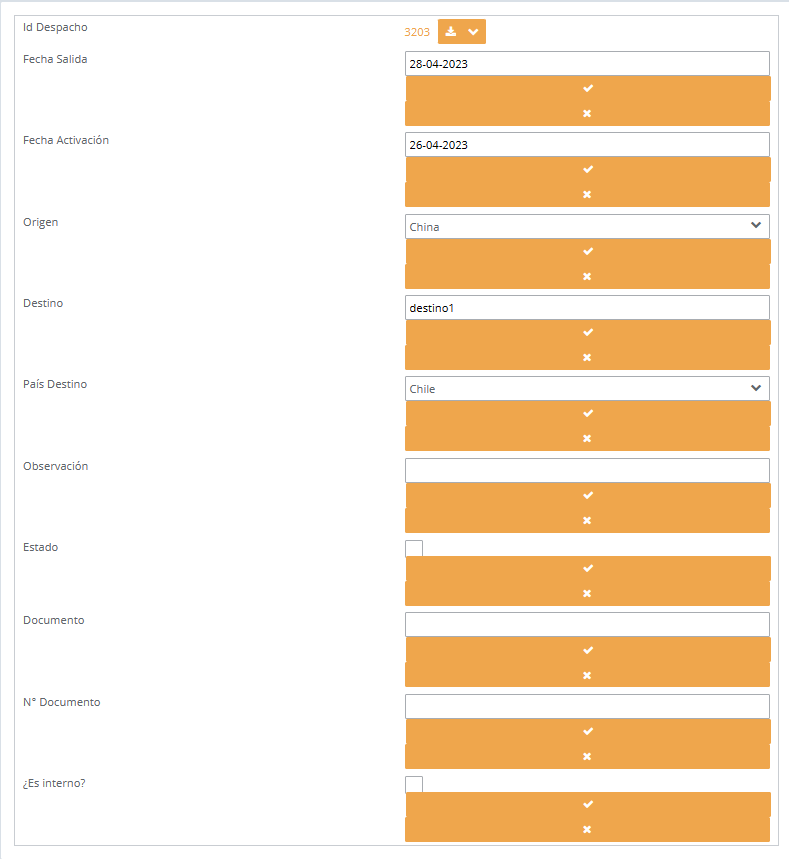
\includegraphics[width=0.8\textwidth]{dm-indv-edit}
	\caption{\label{fig:dm-indv-edit} Edición propiedades despacho. Fuente: Elaboración propia.}
\end{figure}
Existen casos en que no todos los productos deben estar en un mismo despacho y se crean despachos apartes para estos, con el mismo destino y fecha de despacho.
Como en \textit{Operations} el despacho es individual, no existe una forma de agrupar estos despachos que comparten propiedades. Por esto, se plantea crear la funcionalidad de 'Despacho múltiples'. 
Los despachos múltiples tendrán una sección aparte en \textit{Operations}, en el menú lateral los despachos se dividirán entre individuales y múltiples.

Al entrar a la sección de despachos múltiples, se muestra la tabla de los despachos múltiples (figura \ref{fig:dm-mantenedor-mult}) que contiene:
\begin{itemize}
    \item Listado de Despachos Múltiples. Las columnas que se muestran son:
    \begin{itemize}
        \item \textbf{ID de Despacho}
        \item \textbf{Fecha de salida} (Ordenable)
        \item \textbf{Destino} (con filtro de texto)
        \item \textbf{Observación}
        \item \textbf{Estado} (con filtro seleccionado el estado Abierto/Cerrado/Todos)
    \end{itemize}
    \item Botónes de acción en \textit{header} y \textit{footer} para: crear, ver y eliminar despacho.
    \begin{itemize}
        \item \textbf{Crear:} Abre el formulario para crear un despacho múltiple.
        \item \textbf{Ver:} Al seleccionar una fila de la tabla, que corresponde a un despacho, hacer click en esta acción lleva a la vista del despacho múltiple.
        \item \textbf{Eliminar:} Al seleccionar una fila de la tabla, que corresponde a un despacho, hacer click en esta acción elimina el despacho seleccionado (luego de confirmar la acción en un diálogo de confirmación).
    \end{itemize}
    \item Filtro de rango de fechas.
\end{itemize}

\begin{figure}[H]
	\centering
	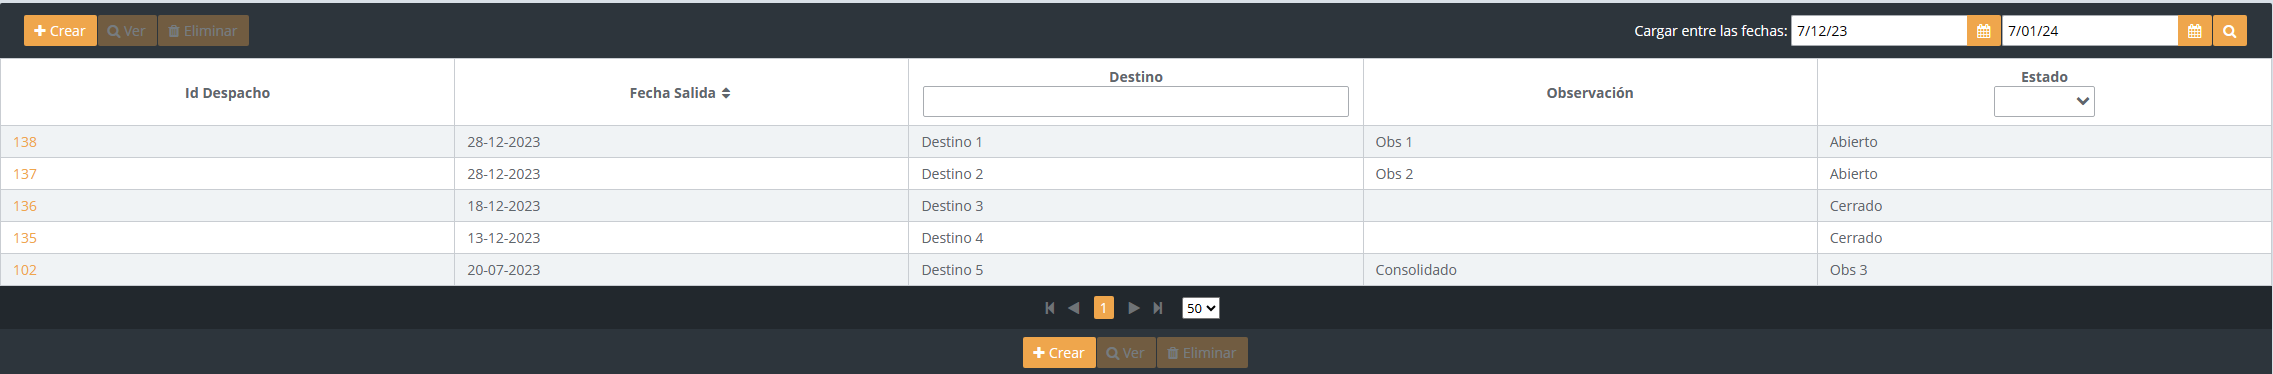
\includegraphics[width=0.8\textwidth]{dm-mantenedor-mult}
	\caption{\label{fig:dm-mantenedor-mult} Sección de despachos múltiples. Fuente: Elaboración propia.}
\end{figure}

En el formulario de creación (figura \ref{fig:dm-create-multi-form}) se ingresan las siguientes propiedades:
\begin{itemize}
    \item Fecha de salida
    \item Destino
    \item País Destino
    \item Observación (propia del despacho padre)
    \item Despacho interno \textit{flag}    
    \item Número de despachos
\end{itemize}

\begin{figure}[H]
	\centering
	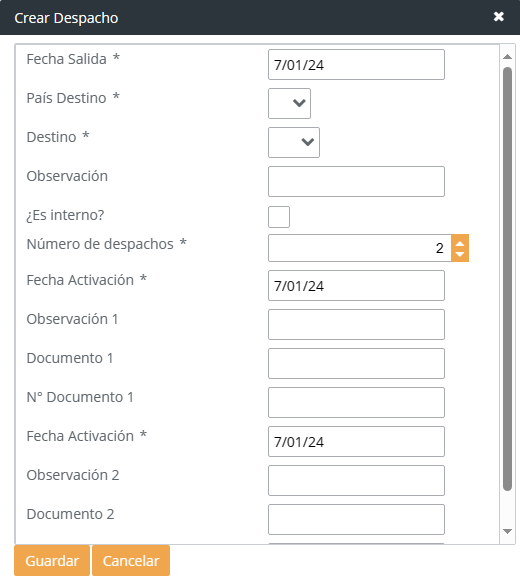
\includegraphics[width=0.5\textwidth]{dm-create-multi-form}
	\caption{\label{fig:dm-create-multi-form} Formulario creación despacho múltiple. Fuente: Elaboración propia.}
\end{figure}

Según el número de despachos hijos ingresado, en el formulario se van agregando campos para cada despacho hijo, diferenciado por un número de creación. Las propiedades individuales de cada despacho hijo son:
\begin{itemize}
    \item Fecha de activación
    \item Observación
    \item Documento
    \item Número de Documento
\end{itemize}

Al guardar el despacho múltiple, las propiedades ingresadas para el despacho padre, son heredadas por los despachos hijos (excluyendo la observación).

Al entrar a la vista de un despacho múltiple (figura \ref{fig:dm-view}) se verá lo siguiente en primera instancia:

\begin{figure}[H]
	\centering
	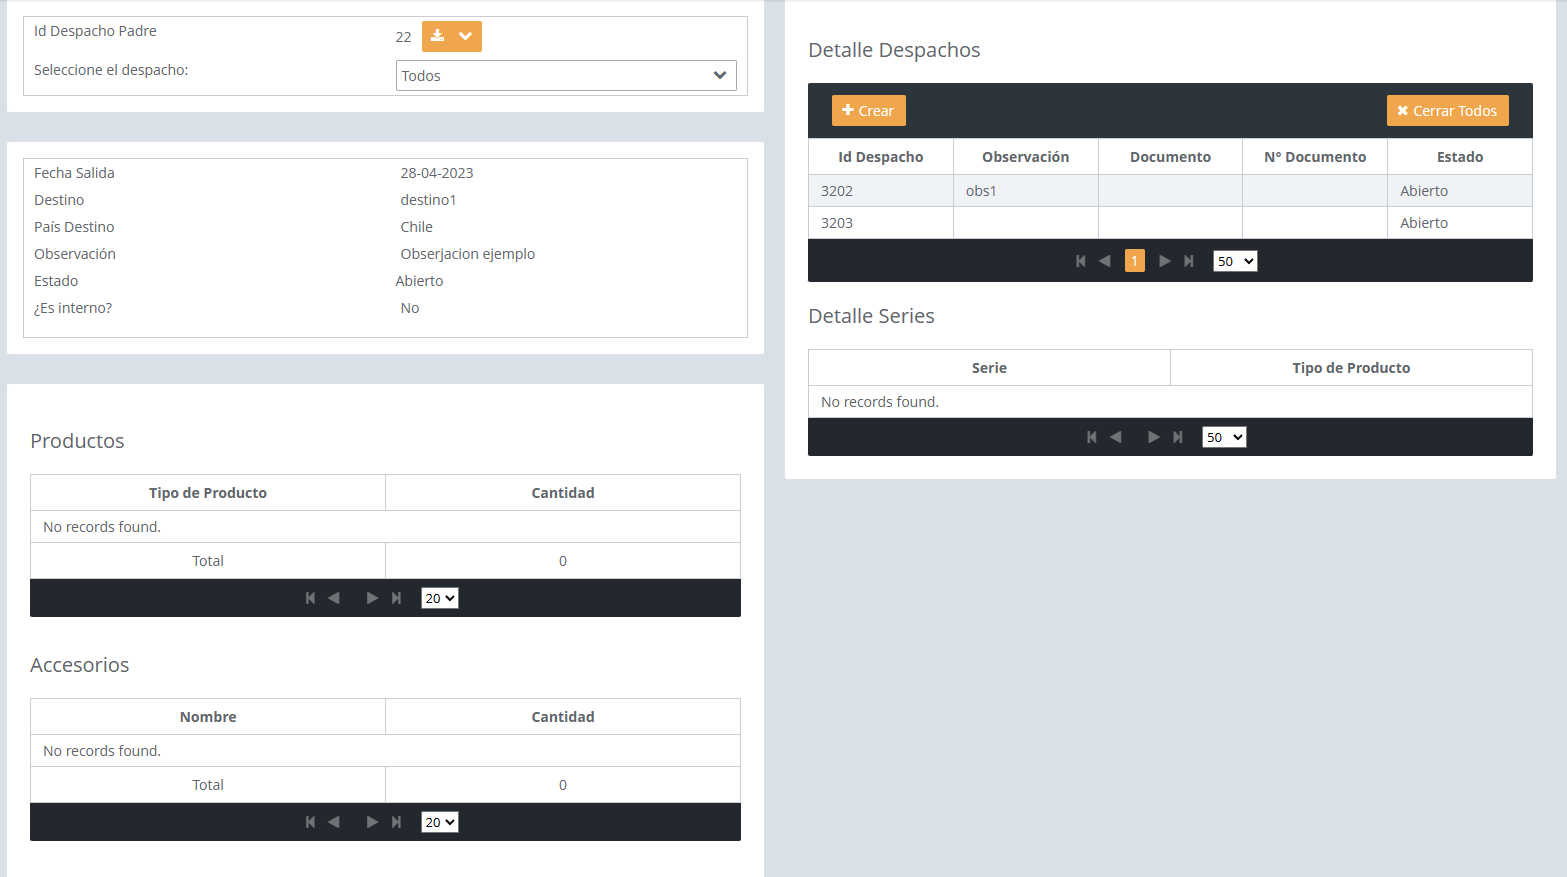
\includegraphics[width=0.8\textwidth]{dm-view}
	\caption{\label{fig:dm-view} Vista despacho múltiple. Fuente: Elaboración propia.}
\end{figure}

\begin{itemize}
    \item Lado izquierdo:
    \begin{itemize}
        \item La primera sección contiene:
        \begin{itemize}
            \item ID del despacho padre, junto a un botón para descargar el reporte del despacho.
            \item Selector de despachos. Al seleccionar la opción 'Todos' se muestra la vista del despacho padre. Si se selecciona la ID de un despacho hijo, se muestra la vista de ese despacho de manera similar a la vista de un despacho individual, como en la figura \ref{fig:dm-child-selected}, pero manteniendo el selector de despachos, y se podrán manejar el despacho como si fuera un despacho individual.
        \end{itemize}
        \item Información del despacho padre. La propiedades son editables.
        \item Tabla de productos: Muestra la cantidad de productos ingresados en todos los despachos hijos.
        \item Tabla de accesorios: Muestra la cantidad de accesorios ingresados en todos los despachos hijos.
    \end{itemize}
    \item Lado derecho:
    \begin{itemize}
        \item Detalle de despachos: Tabla que muestra los despachos hijos. En el \textit{header} de la tabla tiene botones para crear un nuevo despacho (se abre un formulario con las propiedades del despacho individual) y para cerrar todos los despachos.
        \item Detalle de series: Tabla que muestra todas las series de los productos ingresados a los despacho hijos.
    \end{itemize}
\end{itemize}

\begin{figure}[H]
	\centering
	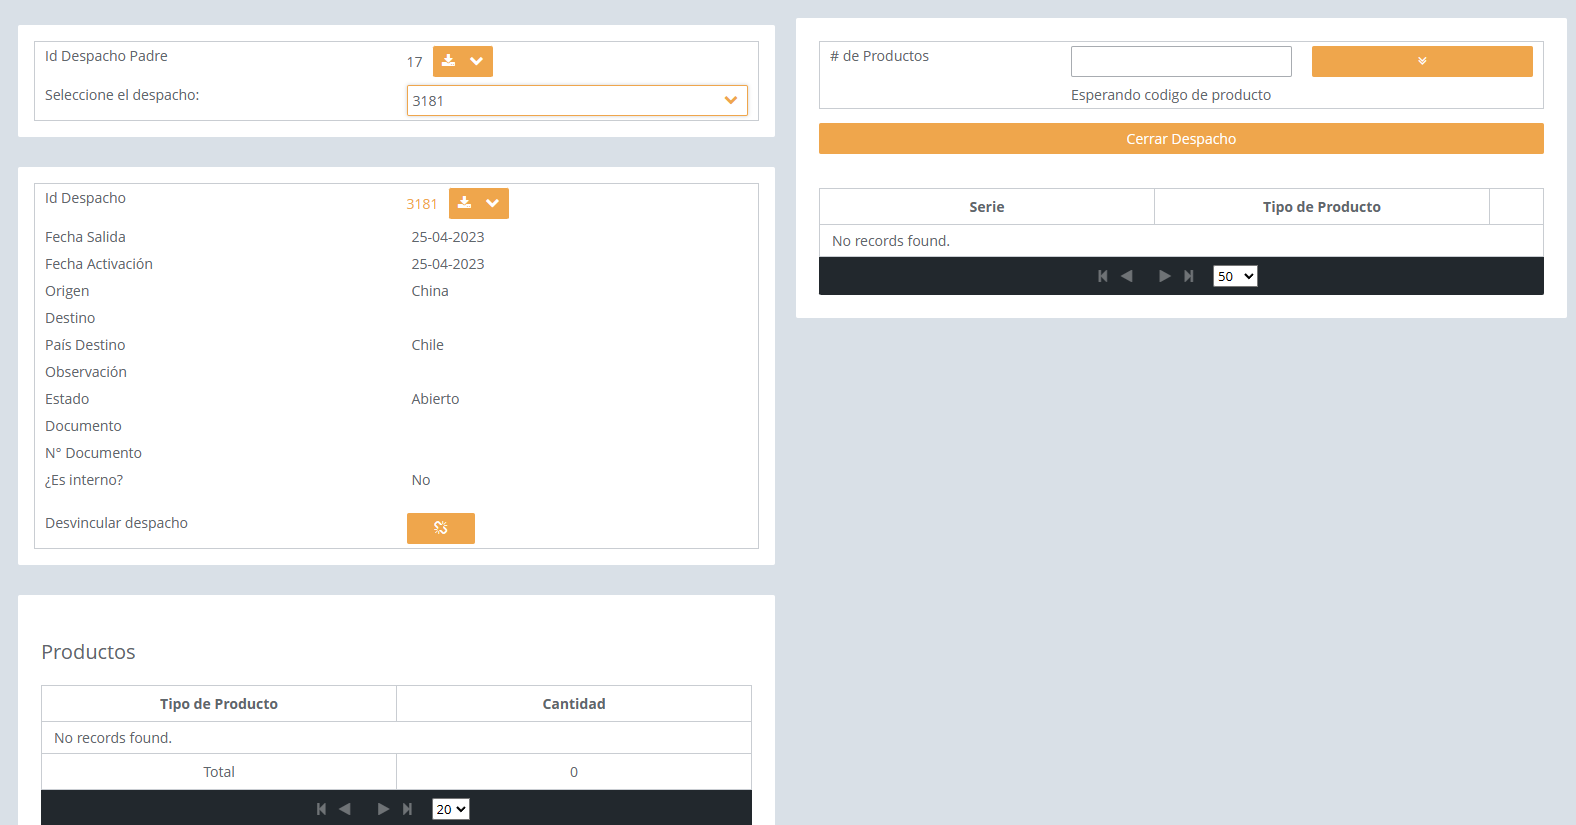
\includegraphics[width=0.8\textwidth]{dm-child-selected}
	\caption{\label{fig:dm-child-selected} Vista despacho hijo seleccionado. Fuente: Elaboración propia.}
\end{figure}


En la vista del despacho múltiple, en la tabla de despachos, se pueden cerrar todos los despachos con el botón 'Cerrar Todos' (figura \ref{fig:dm-close}). Como también se pueden crear nuevos despachos con el botón 'Crear' (figura \ref{fig:dm-create-indv-full}).

\begin{figure}[H]
	\centering
	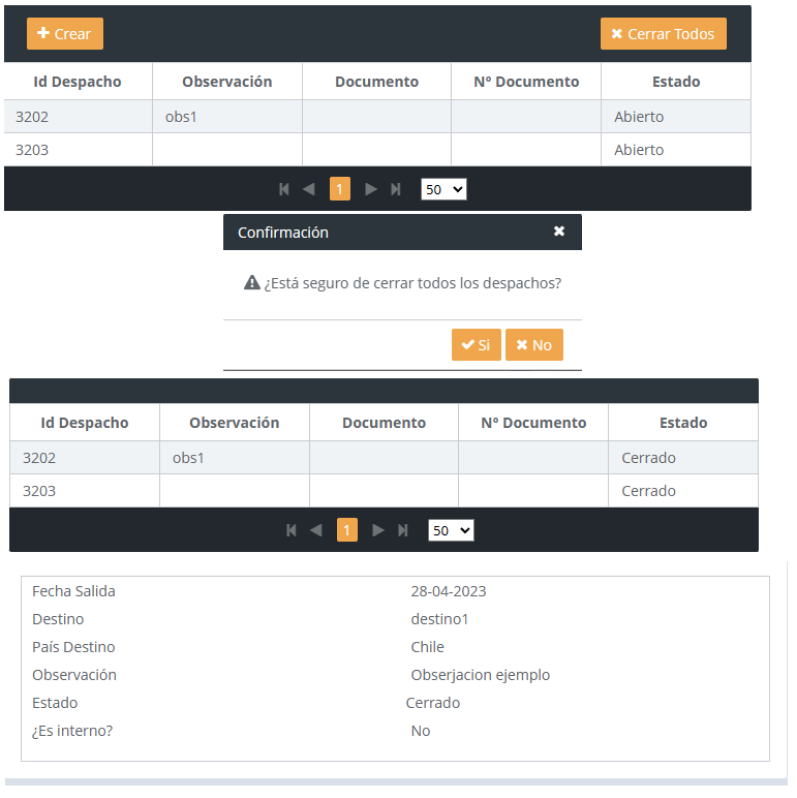
\includegraphics[width=0.8\textwidth]{dm-close}
	\caption{\label{fig:dm-close} Cerrar los despachos desde la tabla. Fuente: Elaboración propia.}
\end{figure}

\begin{figure}[H]
	\centering
	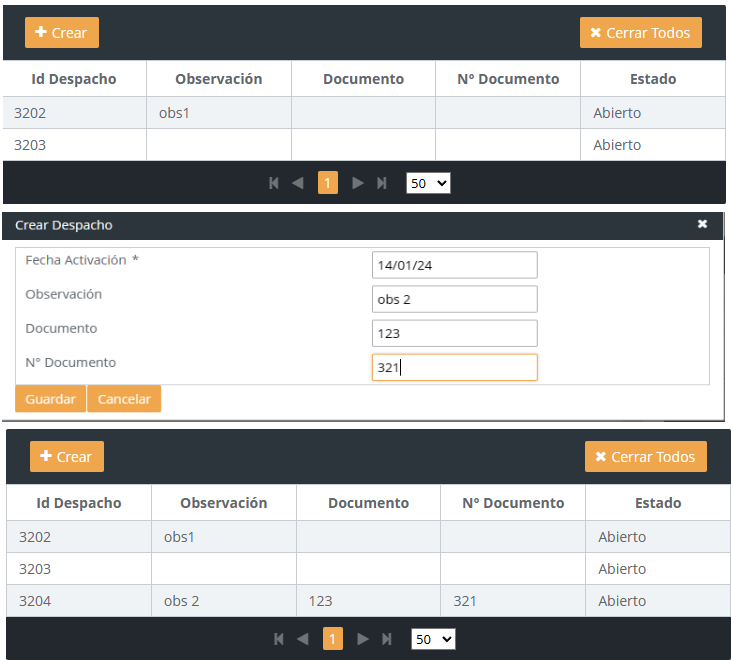
\includegraphics[width=0.8\textwidth]{dm-create-indv-full}
	\caption{\label{fig:dm-create-indv-full} Crear despachos desde la tabla. Fuente: Elaboración propia.}
\end{figure}

Las siguientes propiedades del Despacho Múltiple padre son heredadas por los despachos hijos, por lo que, al editar una de estas propiedades, ya sea desde el despacho padre o del despacho hijo, se actualizarán para los demás despachos hijos y/o padre:
\begin{itemize}
    \item Fecha de salida.
    \item Destino.
    \item País Destino.    
    \item Despacho interno \textit{flag}.    
    \item Estado del despacho (Abierto/Cerrado).
\end{itemize}

El estado del despacho padre depende de los despachos hijos, si todos los despachos hijos están cerrados, entonces el despacho padre está cerrado. En el caso de que haya al menos un despacho hijo abierto, el despacho padre aparece abierto. Mismo caso ocurre con la \textit{flag} de despacho interno.

En la vista de despacho individuales, al entrar en un despacho, en la sección de información se agrega un nueva propiedad 'Id Despacho Padre' que, como dice el nombre, indica la ID del despacho padre. Al hacer click sobre este Id redireccionará a la vista del despacho padre en Despacho Múltiples.
Al lado de esta ID, hay un botón que permite desvincular el despacho del despacho padre (figura \ref{fig:dm-remove-child}). 
En el caso que el despacho no pertenezca a un despacho múltiple, se podrá ingresar la ID de un despacho padre para vincularlo a este (figura \ref{fig:dm-add-indv}). Solo se podrá vincular un despacho individual a un despacho múltiple si las propiedades del despacho múltiple coinciden con el despacho individual.

\begin{figure}[H]
	\centering
	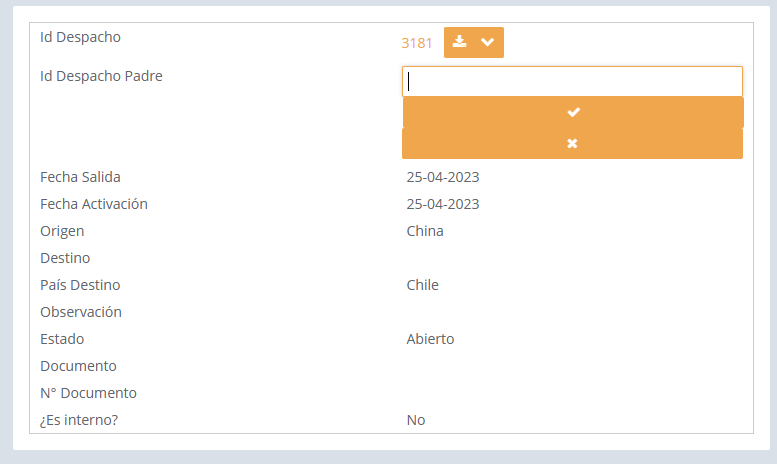
\includegraphics[width=0.8\textwidth]{dm-add-indv}
	\caption{\label{fig:dm-add-indv} Asignar despacho a un despacho múltiple. Fuente: Elaboración propia.}
\end{figure}

\begin{figure}[H]
	\centering
	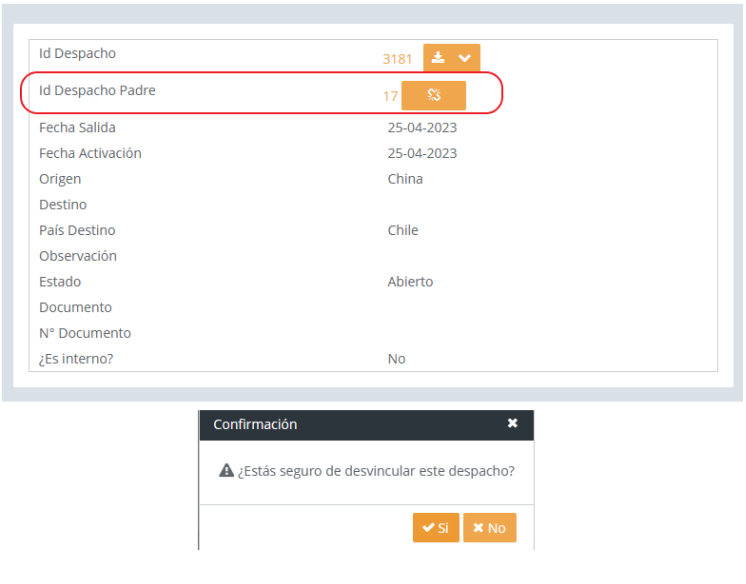
\includegraphics[width=0.8\textwidth]{dm-remove-child}
	\caption{\label{fig:dm-remove-child} Remover de despacho múltiple. Fuente: Elaboración propia.}
\end{figure}

Los despachos múltiples ayudarán a mantener agrupados despachos que comparten ciertas propiedades y poder manejarlas en un mismom lugar.\fi

\subsubsubsection{ACTUALIZACIÓN MASIVA DE PRODUCTOS}

El área de producción al hacer el testeo del hardware y si existe un fallo, se debe dejar el registro en el historial del producto en \textit{Operations}.
Cada producto tiene asociado un historial, las historias del historial se pueden agregar de forma manual o de forma automática realizando ciertas acciones como agregar un producto a un despacho.
Los tipos de historia que se pueden crear de forma manual son:
\begin{itemize}
    \item Observación.
    \item Fallo PrePorducción.
    \item Fallo PostProducción.
\end{itemize}

Para las historias de fallo, se debe ingresar el tipo de falla.

Debido a que se hacen pruebas a muchos productos, el ir agregando el registro a cada producto de manera individual tomaría mucho tiempo para los trabajadores.

Es por esto que se plantea hacer una nueva herramienta en \textit{Operations} que permita poder hacer una actualización masiva de productos para agregar registros al historial de los productos y bloquearlos si es necesario.

Esta nueva herramienta estará en el menú lateral de \textit{Operations} (figura \ref{fig:history-menu}). Esta herramienta (figura \ref{fig:history-view}) consta de dos secciones: Formulario de registro (lado izquierdo) y tabla de productos (lado derecho).

\begin{figure}[H]
	\centering
	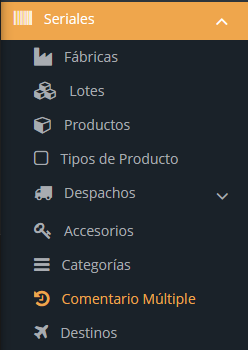
\includegraphics[width=0.5\textwidth]{history-menu}
	\caption{\label{fig:history-menu} Sección de Comentario Múltiple en el menú. Fuente: Elaboración propia.}
\end{figure}

\begin{figure}[H]
	\centering
	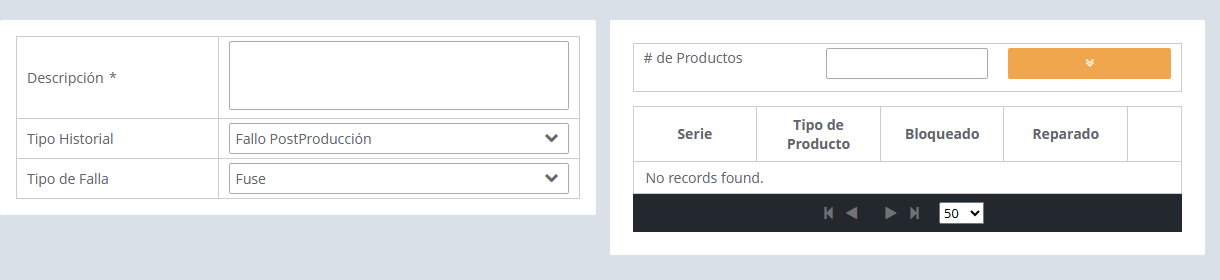
\includegraphics[width=0.8\textwidth]{history-view}
	\caption{\label{fig:history-view} Vista de Comentario Múltiple. Fuente: Elaboración propia.}
\end{figure}

El formulario de registro contiene (figura \ref{fig:history-form}):
\begin{itemize}
    \item Un \textit{TextArea} para ingresar un comentario.
    \item Selector \textit{dropdown} para el tipo de historia.
    \item En caso de seleccionar un tipo de historia de fallo, se desplegará otro selector \textit{dropdown} para escoger el tipo de fallo.
    \item Botón para guardar los registros.
\end{itemize}

\begin{figure}[H]
	\centering
	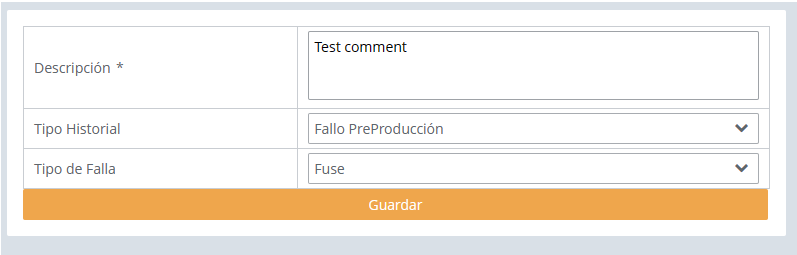
\includegraphics[width=0.8\textwidth]{history-form}
	\caption{\label{fig:history-form} Formulario de registro. Fuente: Elaboración propia.}
\end{figure}

La tabla de productos tendrá lo siguiente (figura \ref{fig:history-table-1}):

\begin{itemize}
    \item Un input donde se ingresará la serie del producto a ingresar.
    \item Tabla de productos, que tiene las siguientes columnas:
    \begin{enumerate}
        \item Serie del producto.
        \item Checkbox para (des)bloquear el producto.
        \item Si se escoge tipo de historia de fallo en el formulario, se mostrará un nueva columna para indicar si el producto está reparado o no, con un \textit{checkbox}.
        \item Botón para eliminar el producto de la tabla.
    \end{enumerate}    
\end{itemize}

\begin{figure}[H]
	\centering
	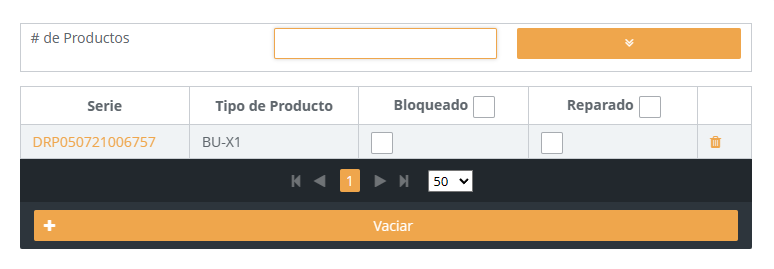
\includegraphics[width=0.8\textwidth]{history-table-1}
	\caption{\label{fig:history-table-1} Tabla de productos. Fuente: Elaboración propia.}
\end{figure}

Al guardar los registros, se abrirá un diálogo de confirmación para guardar la historia (figura \ref{fig:history-create}). Si se entra a la vista de alguno de los productos ingresados, se mostrará la historía en la tabla de historial y según como se seleccionó en la tabla mostrará si está bloqueado o no (figura \ref{fig:history-product}).

\begin{figure}[H]
	\centering
	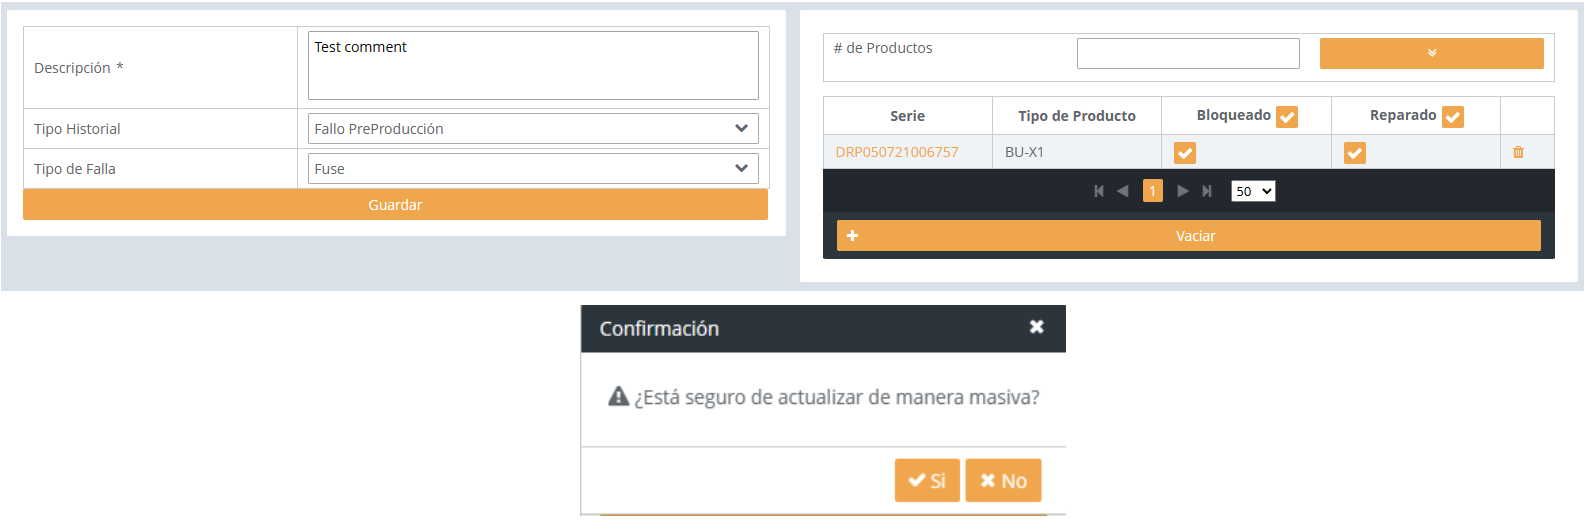
\includegraphics[width=0.8\textwidth]{history-create}
	\caption{\label{fig:history-create} Guardar historia. Fuente: Elaboración propia.}
\end{figure}

\begin{figure}[H]
	\centering
	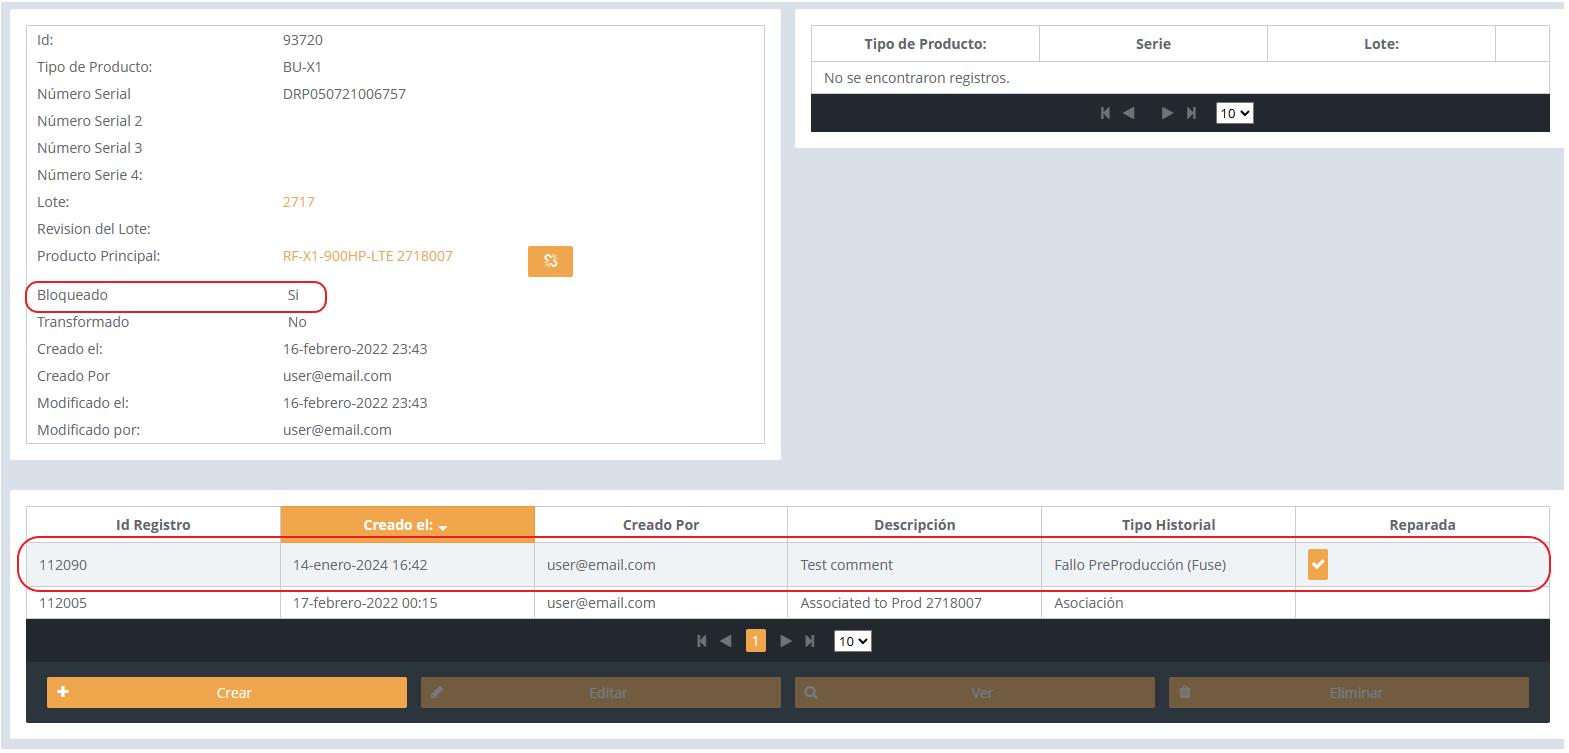
\includegraphics[width=0.8\textwidth]{history-product}
	\caption{\label{fig:history-product} Producto con historia registrada. Fuente: Elaboración propia.}
\end{figure}

\iffalse
\subsubsection{CERTIFICADOS TESTBED}

Dentro de las tareas que cumple el área de producción es son las pruebas del hardware, cada prueba queda documentada con
un certificado en donde se indica si el hardware pasó o no las pruebas para seguir con su producción. Estos certificados son
almacenados en un servidor FTP que después se guardan en un bucket de S3.

La aplicación de \textit{Operations} es para la gestión de lotes y despachos de productos, además de la edición de productos.
El producto tiene un historial con historias asociadas que indican ingresos a lotes, despachos, marcar como producto fallado y/o reparado.

Los trabajadores para acceder a los certificados testbed...

Teniendo esto en cuenta, se plantea implementar un modo que agregue al historial del producto testeado un registro junto con el certificado Testbed en \textit{Operations}.

En \textit{Operations}, los productos tienen un historial de movimientos, acciones (creación, ingreso a despacho, etc.), registro de fallos/arreglos, entre otros.
Un registro en el historial contiene el tipo de historia, fecha, usuario y descripción. Dentro de los tipos de historia están:
\begin{itemize}
    \item Fallo Pre-Producción
    \item Fallo Post-Producción
\end{itemize}

Para solucionar esta problemática, se va a agregar un nuevo tipo de historia llamado 'Certificados Testbed' para registrar los certificados testbed, valga la redundancia, de los productos.
Esta historia se registrará automáticamente cuando el trabajador de taller que esté probando los productos suba los certificados a un servidor FTP. Los certificados en este servidor se respaldan en un \textit{bucket} de S3 en \textit{Amazon Web Services}.
Cada vez que se agregue un certificado al \textit{bucket}, se activa una función \textit{Lambda} que guardará en la base de datos de \textit{Operations} en una nueva tabla creada para los certificados.

Las columnas de la tabla de certificados en la base de datos son las siguientes: 
\begin{itemize}
    \item Fecha.
    \item Llave del objeto en el \textit{bucket}.
    \item Serie del producto.
\end{itemize}
Esta tabla tendrá un \textit{trigger} que se activará el ingresar un nuevo registro, que creará la historia si y solo si el producto está creado en \textit{Operations}.
En el caso que el producto aún no haya sido ingresado en \textit{Operations}, la historia se agregará cuando se cree el producto con un \textit{trigger} en la tabla de productos.
Estas historias no se podrán editar ni eliminar.

En el historial del producto, la historia de certificados mostrará en la descripción un \textit{presigned URL} con el certificado.

Teniendo estas historias de certificados, se agregará una restricción en los despachos, el cuál no se permitirá ingresar un producto que no tenga un certificado testbed.
\fi

\subsubsection{DROPCONTROL}

\textit{DropControl} es el software principal de \textit{WiseConn}, en el cual el usuario puede operar, monitorear y gestionar múltiples procesos agrícolas en los campos.
Algunas de las herramientas disponibles están\footnote{\href{https://wiseconn.com/cl/nuestra-solucion/}{\textit{WiseConn: Nuestra Solución.}}}:
\begin{itemize}
    \item \textbf{Programación de Riego y Fertirriego}
    \SubItem{Herramienta para programación de riego y fertirriego, sistemas de filtrado y VDF.}
    \SubItem{Reportes de riego, nutrición por equipo y sectores de riego.}
    \SubItem{Integración de amplia gama de sensores y actuadores.}
    \item \textbf{Análisis de Clima}
    \SubItem{Datos climatológicos (horas frío, grados día, Et0, entre otros).}
    \SubItem{Reportes de Balance Hídrico}
    \SubItem{Integra servicios de pronóstico de clima.}
    \item \textbf{Graficador Libre}
    \SubItem{Comparación de múltiples variables entre sí y contraste con temporadas pasadas.}
    \SubItem{Generar plantillas de gráficos.}
    \SubItem{Descarga de gráficos en formato PDF y extraer datos en Excel.}
    \item \textbf{Análisis de Imágenes}
    \SubItem{Servicio de imágenes satelitales y áreas organizadas por sector de riego.}
    \SubItem{Compara imágenes de NDVI\footnote{\href{https://eos.com/es/make-an-analysis/ndvi/}{NDVI: Índice De Vegetación De Diferencia Normalizada}} (sigla en inglés de Índice de vegetación de diferencia normalizada) de Sentinel-2\footnote{\href{https://www.esa.int/Space_in_Member_States/Spain/SENTINEL_2}{SENTINEL 2}} entre los diferentes sectores del campo con diferentes fechas.}    
\end{itemize}

\subsubsubsection{FÓRMULAS}

Dentro de \textit{DropControl} existe la herramienta de \textit{Dashboard Libre} (Figura \ref{fig:dash-example}), el cual asimila a una pizarra organizada en cuadrillas en el cual se pueden crear y organizar \textit{widgets}.
Los \textit{widgets} disponibles son:
\begin{itemize}
    \item \textbf{Gráfico}: Gráfico de variables seleccionadas por el usuario. Dentro de los aspectos configurables están: agrupación de los datos, configuración de ejes y anotaciones en el gráfico.
    \item \textbf{Tabla}: Tabla de variables seleccionadas por el usuario. Dentro de los aspectos configurables están la agrupación de los datos.
    \item \textbf{Número}: Muestra el valor (último dato, promedio, suma, mínimo o máximo) de una variable seleccionada dentro de un periodo seleccionado.
    \item \textbf{Gráfico de Suelo}: Gráfico de solo variables de suelo, dentro de las que están la humedad, temperatura en distintas profundidades.
    \item \textbf{Tabla de Riegos}: Tabla que muestra las horas de riego en un tiempo determinado en los campos y equipos de riego seleccionado por el usuario.
\end{itemize}

\begin{figure}[H]
	\centering
	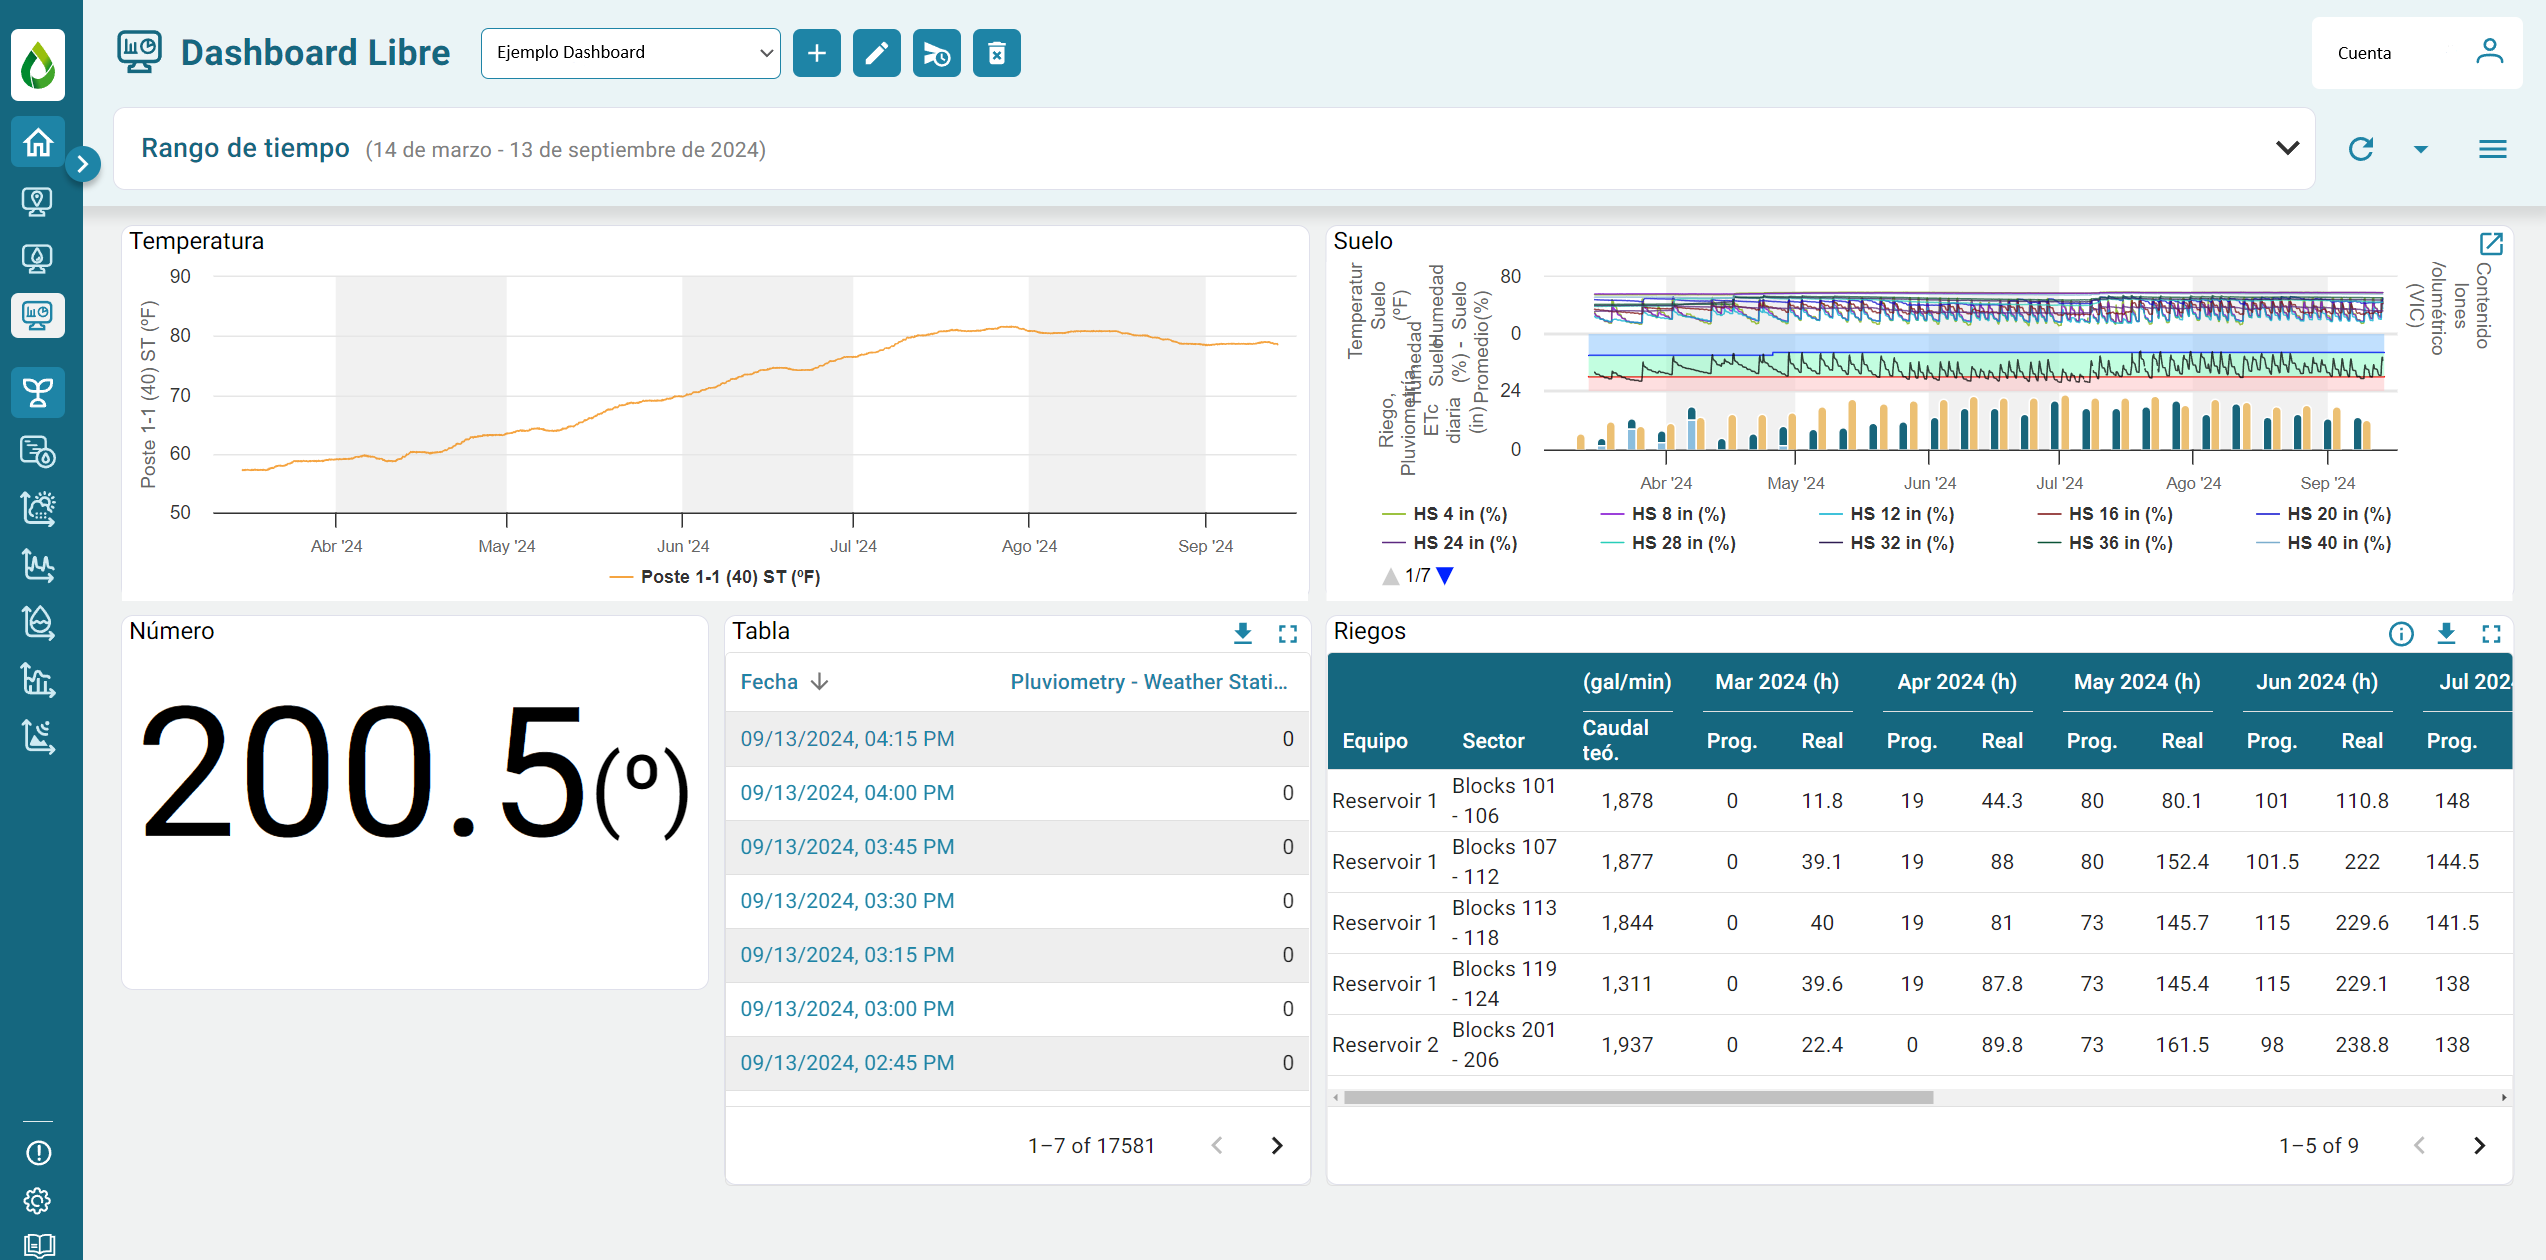
\includegraphics[width=1\textwidth]{widget-formulas/ejemplo-dash-normal}
	\caption{\label{fig:dash-example} Ejemplo de Dashboard Libre. Fuente: Elaboración propia.}
\end{figure}

En \textit{DropControl} cada campo tiene su sistema de unidades asignado según el país del campo. Existen casos en que el usuario quiere ver ciertos datos en otras unidades (ejemplo, ver el volumen de riego en litros en lugar de galones), pero el cambiar las unidades del campo provocaría errores en estimaciones y/o cálculos de riego, es por esto que para estos casos se crean sensores 'virtuales', los cuales toman los datos de otro sensor y transforman los datos según el requerimiento.
El proceso de creación de estos sensores virtuales...

Es por esto que en la herramienta de \textit{Dashboard Libre}, para los \textit{widgets} de gráfico y tabla, se decide implementar una configuración de fórmulas en donde el usuario podrá realizar operaciones utilizando las variables seleccionadas para hacer conversión de unidades y/o crear nuevas variables.
Para esta nueva configuración se toma inspiración de \textit{Amazon CloudWatch}\footnote{\href{https://docs.aws.amazon.com/es_es/AmazonCloudWatch/latest/monitoring/using-metric-math.html}{\textit{Amazon CloudWatch}: Uso de la calculadora de métricas}}, que permite añadir expresiones matemáticas a un gráfico de métricas de \textit{CloudWatch}.

Se implementará solo en los \textit{widgets} de gráfico y tabla, ya que, utilizan el mismo componente y dependiendo de si es un \textit{widget} de tabla o gráfico muestra ciertos \textit{inputs} en la pestaña de \textbf{Ajustes} como muestra en la figuras \ref{fig:variables-table-diff} y \ref{fig:ajustes-table-diff}. Además, en el formulario de gráfico, tiene una pestaña extra de \textbf{Configuración de Ejes} (figura \ref{fig:axis-config-table}), en el cual se pueden configurar \textbf{plotlines/plotbands} y configurar los ejes. Además, el formulario de gráfico permite una previsualización con el botón \textbf{Previsualizar} (figura \ref{fig:preview-grafico}).

\begin{figure}[H]
	\centering
	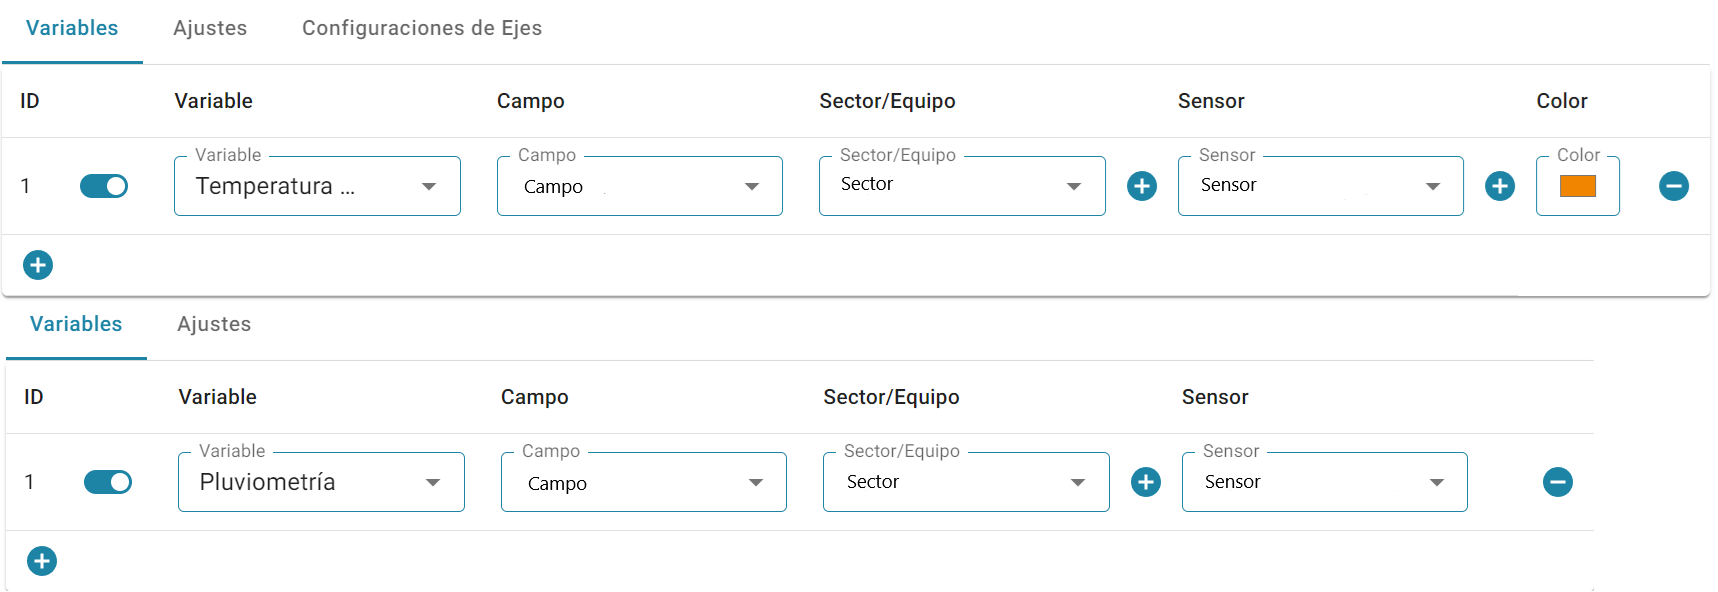
\includegraphics[width=1\textwidth]{widget-formulas/variables-table-diff}
	\caption{\label{fig:variables-table-diff} Diferencias formulario de variables en \textit{widget} de gráfico y tabla. Fuente: Elaboración propia.}
\end{figure}
\begin{figure}[H]
	\centering
	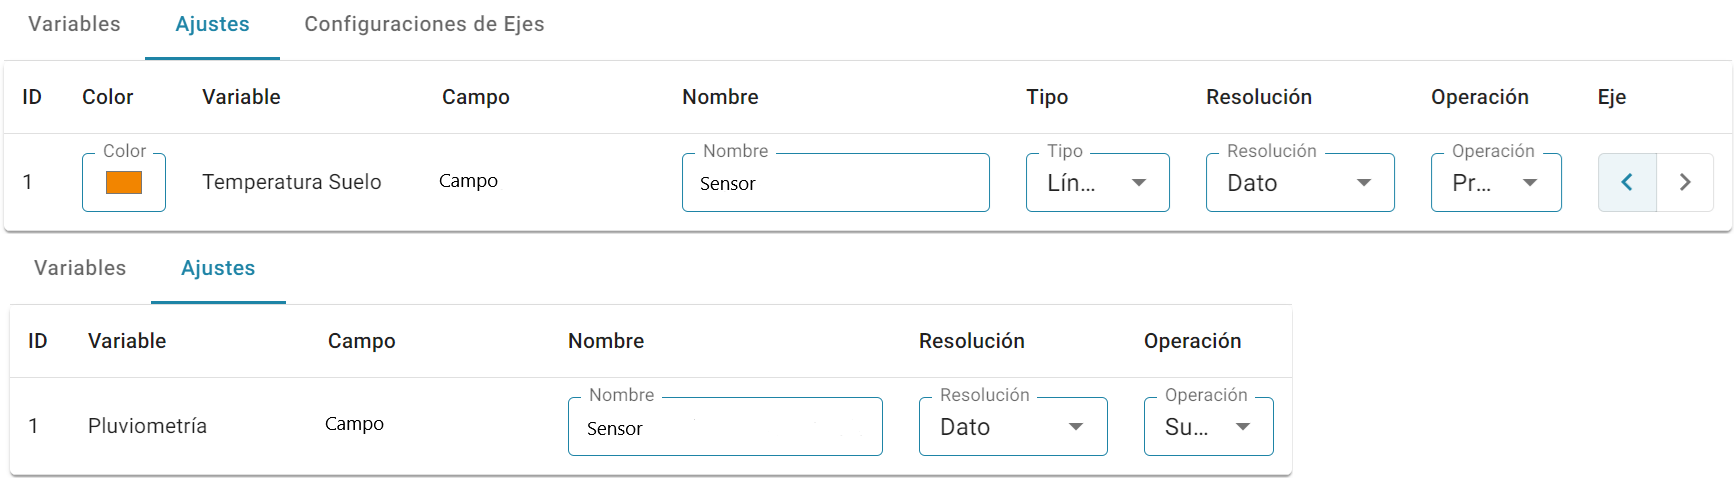
\includegraphics[width=1\textwidth]{widget-formulas/ajustes-table-diff}
	\caption{\label{fig:ajustes-table-diff} Diferencias formulario de ajustes en \textit{widget} de gráfico y tabla. Fuente: Elaboración propia.}
\end{figure}
\begin{figure}[H]
	\centering
	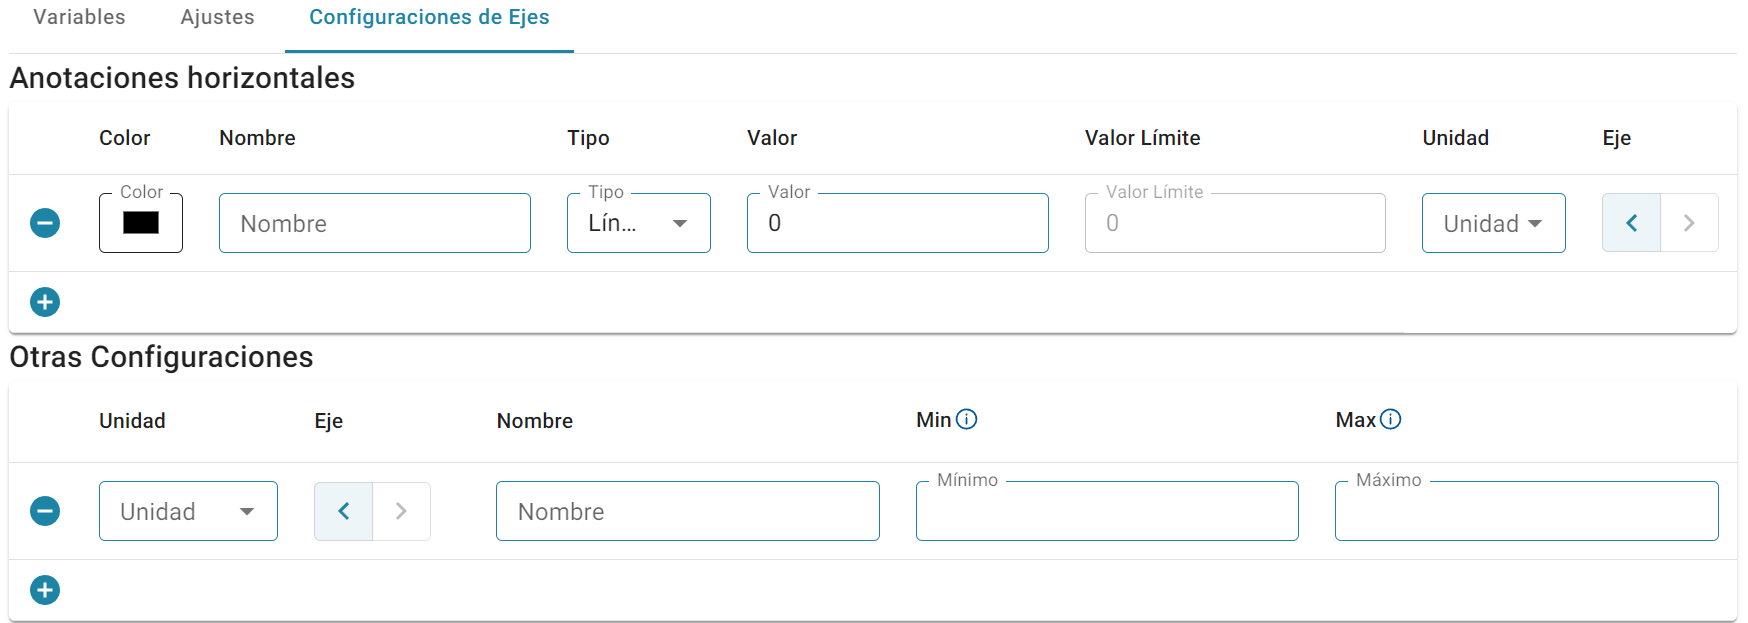
\includegraphics[width=1\textwidth]{widget-formulas/axis-config-table}
	\caption{\label{fig:axis-config-table} Formulario para configuración de ejes, solo presente en \textit{widget} de gráfico. Fuente: Elaboración propia.}
\end{figure}
\begin{figure}[H]
	\centering
	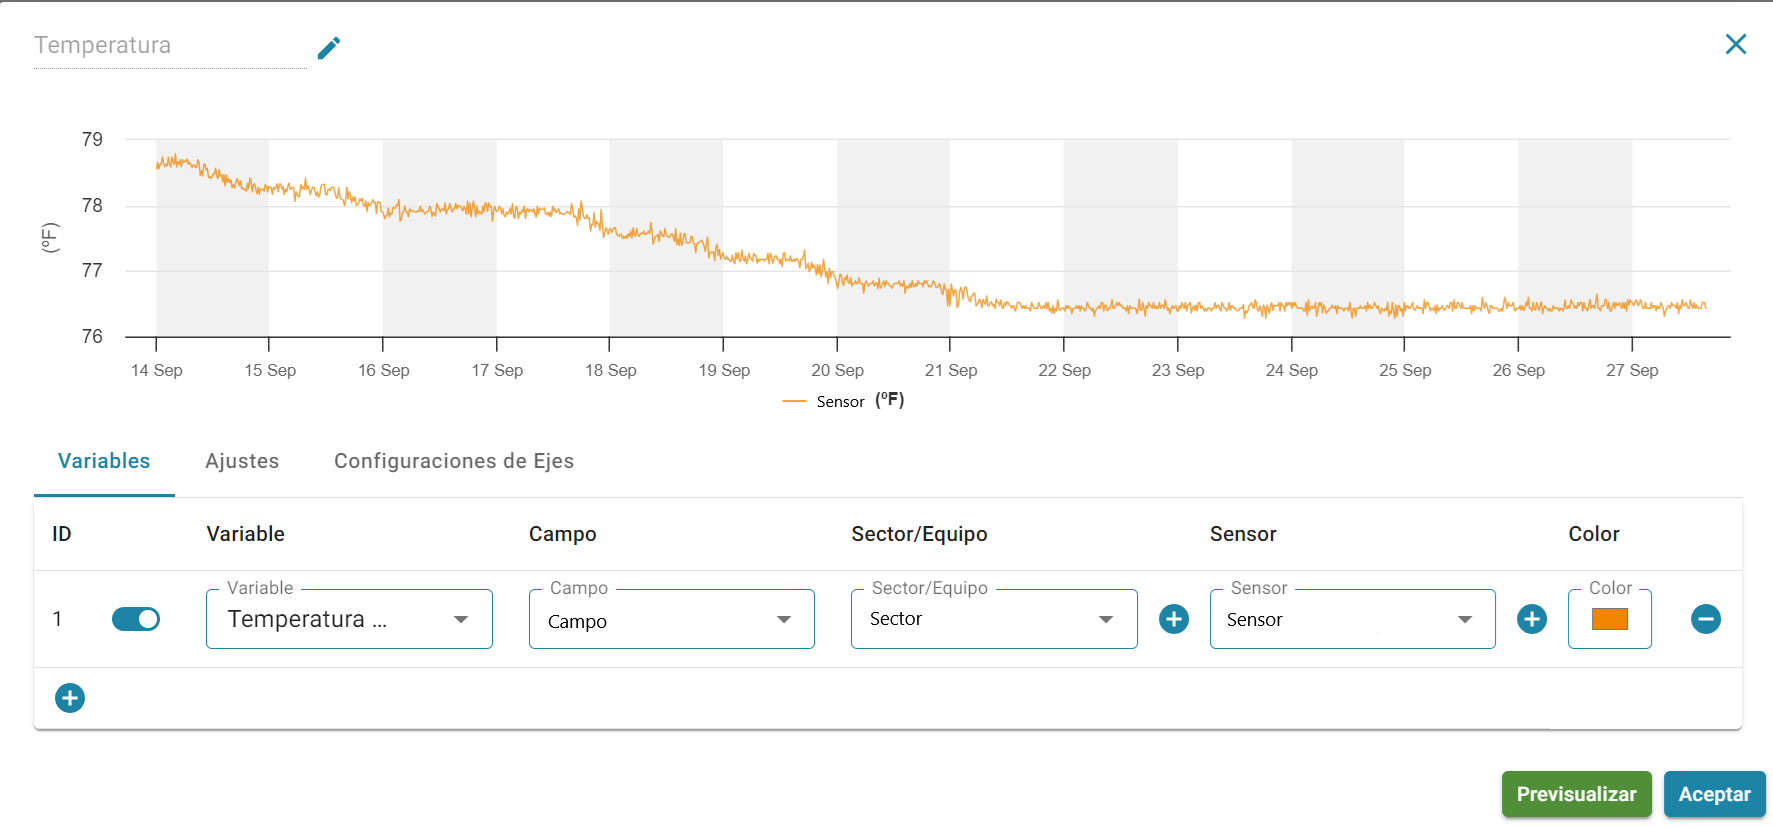
\includegraphics[width=1\textwidth]{widget-formulas/preview-grafico}
	\caption{\label{fig:preview-grafico} Previsualización en formulario de\textit{widget} de gráfico. Fuente: Elaboración propia.}
\end{figure}

En los formularios de creación/edición de los \textit{widgets} de gráfico y tabla se agrega una nueva pestaña con el título de 'Fórmulas'. El formulario presente en esta nueva pestaña tendrá la misma estructura que la pestaña de variables (figura \ref{fig:variables-table-diff}) el formulario de esta sección constará de una tabla que contendrá lo siguiente:
\begin{itemize}
    \item ID de la formula.
    \item \textit{Toogle} para mostrar el resultado de la fórmula en la tabla/gráfico.
    \item \textit{Input} para ingresar el nombre de la fórmula.
    \item \textit{Input} para ingresar la fórmula. Al lado del \textit{input} habrá un botón que desplegará una lista con las variables, fórmulas, operadores, números, separadores de decimales y funciones.
    \item \textit{Input} para ingresar la unidad.
    \item \textit{Input} para ingresar la cantidad de decimales a mostrar.
    \item Selector de color (solo gráfico).
    \item Tipo: línea, barra o apilado (solo gráfico).
    \item Posición del eje (solo gráfico).
    \item Botón para eliminar la fórmula de la tabla.
    \item En el \textit{footer}, un botón para agregar una nueva fila.
\end{itemize}

El formato de las formulas será de la siguiente manera:
\begin{itemize}
    \item Las variables seleccionadas se representaran de la forma D\{ID variable\}.
    \item Se podrán referenciar fórmulas de la misma tabla de la forma F\{ID fórmula\}.
    \item Los operadores serán '+' (suma), '-' (resta), '*' (multiplicación), '/' (división) y '\^{}' (potencia).
    \item Los números no pueden tener separador de miles.
    \item El separador de decimales puede ser con punto o coma.
    \item Dentro de las funciones soportadas están: ...
\end{itemize}

Dentro de los requisitos que debe tener la fórmula para que sea válida:
\begin{itemize}
    \item Debe contener solo caracteres válidos, es decir, la formula debe contener:
        \SubItem{Números. Si son números decimales se debe usar separador de decimales ya sea punto o coma. Los números no deben contener separados de miles.} 
        \SubItem{Operadores matemáticos: '+' (suma), '-' (resta), '*' (multiplicación), '/' (división) y '\^{}' (potencia).}
        \SubItem{Paréntesis.}
        \SubItem{Funciones soportadas.}
    \item La fórmula debe tener al menos una variable o referencia a una fórmula.
    \item No pueden existir referencias circulares\footnote{\href{https://en.wikipedia.org/wiki/Circular_reference}{\textit{Wikipedia - Circular Reference}}} al hacer referencias a otras fórmulas. Esto puede provocar un \textit{loop} y puede afectar el navegador del usuario.
    \item Las variables y fórmulas referenciadas en la fórmula deben existir en el \textit{widget}.        
\end{itemize}

Para ver si la fórmula es válida, se utilizará una expresión regular para ver si la fórmula tiene caracteres válidos.
Para el caso de las referencias circulares, se utilizará \textit{Topological sorting}\footnote{\href{https://en.wikipedia.org/wiki/Topological_sorting}{\textit{Wikipedia - Topological Sorting}}} utilizando el algoritmo de \textit{Depth-first search}\footnote{\href{https://en.wikipedia.org/wiki/Depth-first_search}{\textit{Wikipedia - Depth-first search}}}.
Este algortimo también servirá para obtener el orden en el que las fórmulas deben ser calculadas.

La implementación de \textit{Topological sort} será de la siguiente manera:
\begin{enumerate}
    \item Construir el gráfo de dependencia, es decir, un objeto donde la llave será la ID de la fórmula y el valor será un array con las IDs de las fórmulas referenciadas.
    \item Con el grafo de dependecia, aplicamos \textit{Topological sort} con \textit{Depth-first search}. En el caso de que exista una referencia circular retornará un error con el ID de la formula, caso contrario, entrega un array con el orden de las fórmulas para calcular.
\end{enumerate}

El proceso del cálculo de las formulas será el siguiente:
\begin{enumerate}
    \item Se obtiene los datos de las variables del \textit{backend}. Los datos de cada sensor vienen en un \textit{array} de objetos de \textit{date} (fecha) y \textit{value} (valor).
    \item Parsear la fórmula:
    \SubItem{Reemplazar las comas por punto (separador de decimales).}
    \SubItem{Reemplazar las funciones por las funciones de la librería \textit{Math} de \textit{JavaScript}}
    \SubItem{Se obtienen las variables y fórmulas referenciadas.}
    \SubItem{Con el constructor \textbf{Function()}\footnote{\href{https://developer.mozilla.org/en-US/docs/Web/JavaScript/Reference/Global_Objects/Function/Function}{\textit{Function}}} creamos la función que hará el cálculo de la fórmula donde los argumentos de la función serán las variables y fórmulas referenciadas y la función será la fórmula parseada.}
    \SubItem{En el caso de tener múltiples fórmulas con fórmulas referenciadas, se hace un ordenamiente con el algoritmo \textit{Topological Sort} para obtener el orden de fórmulas a calcular. Con esto primero calculámos las fórmulas sin referencias primero y luego las que contienen referencias}
    \SubItem{Se obtienen los datos de las variables referenciadas de la respuesta del punto 1. Luego se guarda en un objeto para ser reutlizadas por las demás fórmulas}
    \SubItem{En el caso de tener fórmulas referenciadas, se obtienen los datos objeto donde se van guardando los resultados de las fórmulas para ser reutilizadas por las demás fórmulas.}
    \SubItem{Se itera sobre los \textit{arrays} de datos para obtener las fechas y se guardan en un \textit{Set}}
    \SubItem{Se itera sobre el \textit{Set} de fechas. Por cada fecha se obtiene el dato de cada variable/fórmula y se ejecuta la función con la fórmula. En el caso en que en una variable no exista la fecha, no se realiza el cálculo y se continua con la siguiente fecha. En el caso de que en una fecha de resultado de tipo \textit{\textbf{NaN}}, \textit{\textbf{Infinity}} o \textit{\textbf{-Infinity}} se guarda el resultado como \textbf{\textit{null}}.}    
    \SubItem{Se guarda el resultado de la fórmula.}
    \SubItem{Al terminar el cálculo de todas las fórmulas, se crea la serie para el gráfico o columna para la tabla (dependiendo del \textit{widget}).}
\end{enumerate}

Como se muestra en el proceso del cálculo, el cálculo de hace fecha a fecha de los datos. Si las variables tienen datos desfasados el cálculo no dará resultado, es por esto que en la pestaña de \textbf{Ajustes} el usuario debe cambiar la resolución de datos de las variables para que las fechas de los datos coincidan, como se muestra en la figura \ref{fig:dash-settings-res}.
Esto también se utilza para validar la fórmula, evaluando las fórmulas con valor 1 en todas las variables. En el caso que la fórmula no entregue un resultado de tipo \textbf{\textit{number}} de \textit{JavaScript}, la fórmula es considerada inválida.

\begin{figure}[H]
	\centering
	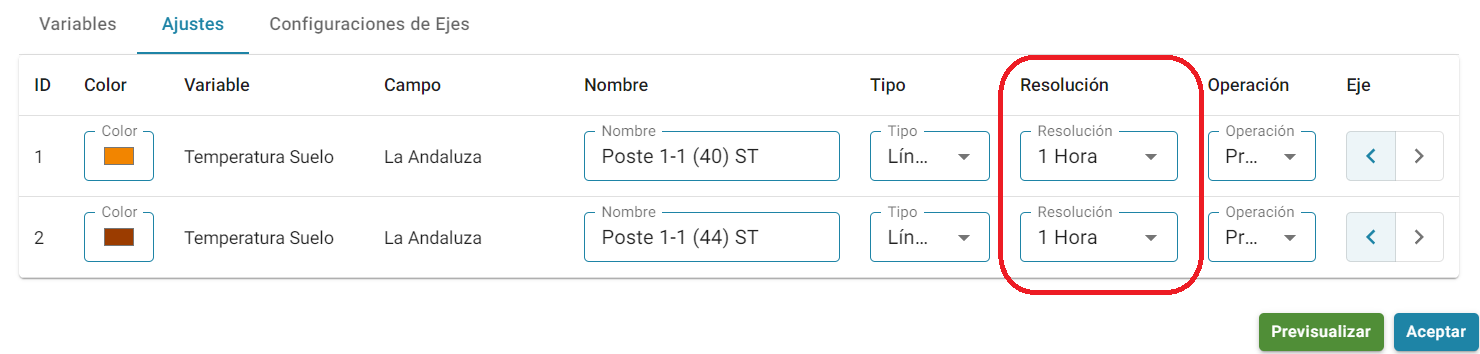
\includegraphics[width=0.8\textwidth]{widget-formulas/dash-settings-res}
	\caption{\label{fig:dash-settings-res} Resolución de datos en formulario de gráfico/tabla. Fuente: Elaboración propia.}
\end{figure}

\iffalse
\subsubsection{SETUP}

\textit{SETUP} es una herramienta interna utilizada por el área de soporte en donde se realizan configuraciones de cuentas, campos, sectores, usuarios, entre otros.

\subsubsubsection{CONFIGURADOR DE FUENTES}

Una de las herramientas más recientes que se ofrece en \textit{DropControl} es el Análisis de Fuentes. En esta herramienta se pueden visualizar las distintas fuentes de agua de un campo como el tranque, canal, equipo de riego e impulsión.
Para mostrar las fuentes de agua en la herramienta, se deben realizar las configuraciones de las fuentes de agua y las conexiones entre ellas en la aplicación de \textit{SETUP}.

Para realizar estas configuraciones se decidió crear un configurador gráfico, donde se agregan 'nodos' a una 'pizarra'. Estos nodos tienen puertos de entrada y salida, donde se conectaran con los demás fuentes de agua. Al hacer click sobre sobre estos nodos, se abrirá un formulario donde se agregan las configuraciones de la respectiva fuente de agua.

Esta configuración tiene una segunda fase, donde luego de guardar los cambios del configurador gráfico, se puede configurar las coordenadas de las fuentes de agua de forma manual o haciendo click en el mapa.

Este configurador gráfico está disponible en la configuración \textit{Wizard} de \textit{SETUP}, en el paso de 'Otras configuraciones' existirá una opción de configuración bajo el nombre 'Configuración de fuentes'.
Al seleccionar esta nueva configuración (figura \ref{fig:water-view}), se despliega una 'pizarra' en la cual se puede realizar la configuración de fuentes del campo, mediante la creación de un diagrama. El diagrama los siguientes elementos (figura \ref{fig:water-nodes-board}):
\begin{itemize}
    \item \textbf{Metrahidráulicas (Fuentes de agua):} Estos serían los nodos del diagrama. Dentro de las metrahidráulicas disponibles están:
          \begin{itemize}
              \item Canal
              \item Equipo
              \item Impulsión
              \item Tranque
              \item Pozo
          \end{itemize}   
\end{itemize}

\begin{figure}[H]
	\centering
	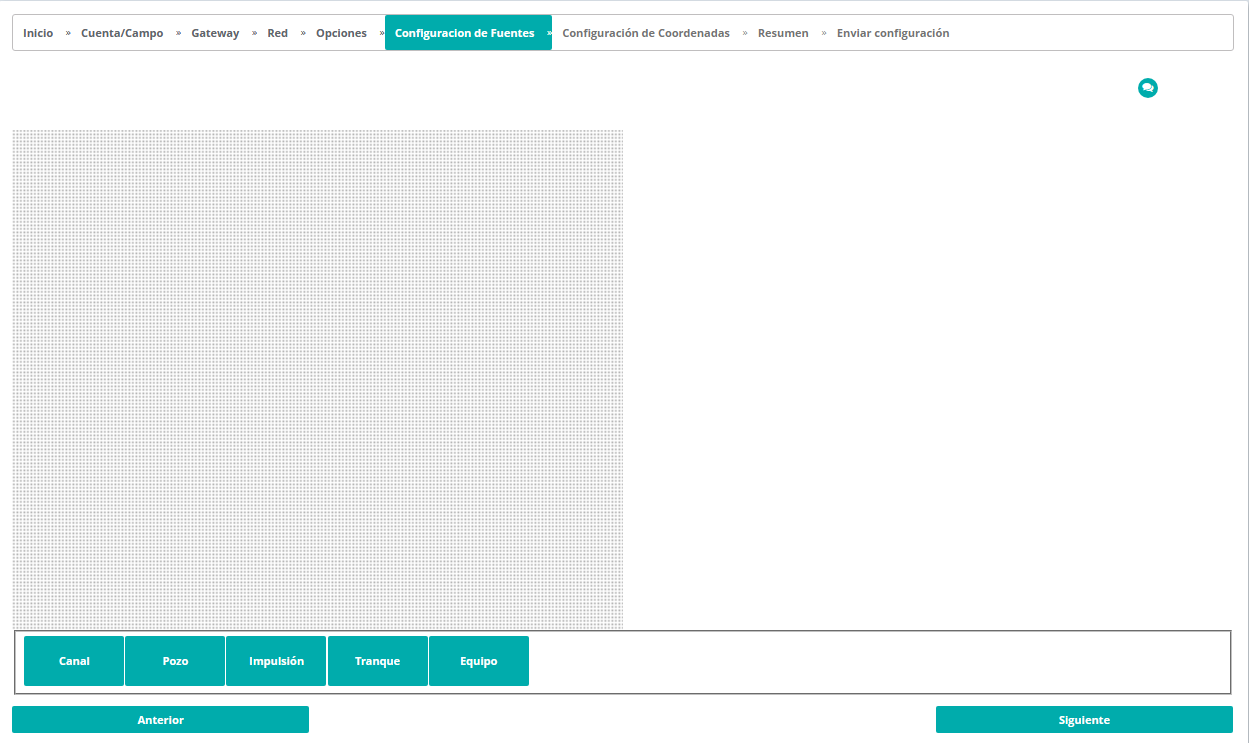
\includegraphics[width=0.8\textwidth]{water-view}
	\caption{\label{fig:water-view} Vista de Configurador de fuentes. Fuente: Elaboración propia.}
\end{figure}

\begin{figure}[H]
	\centering
	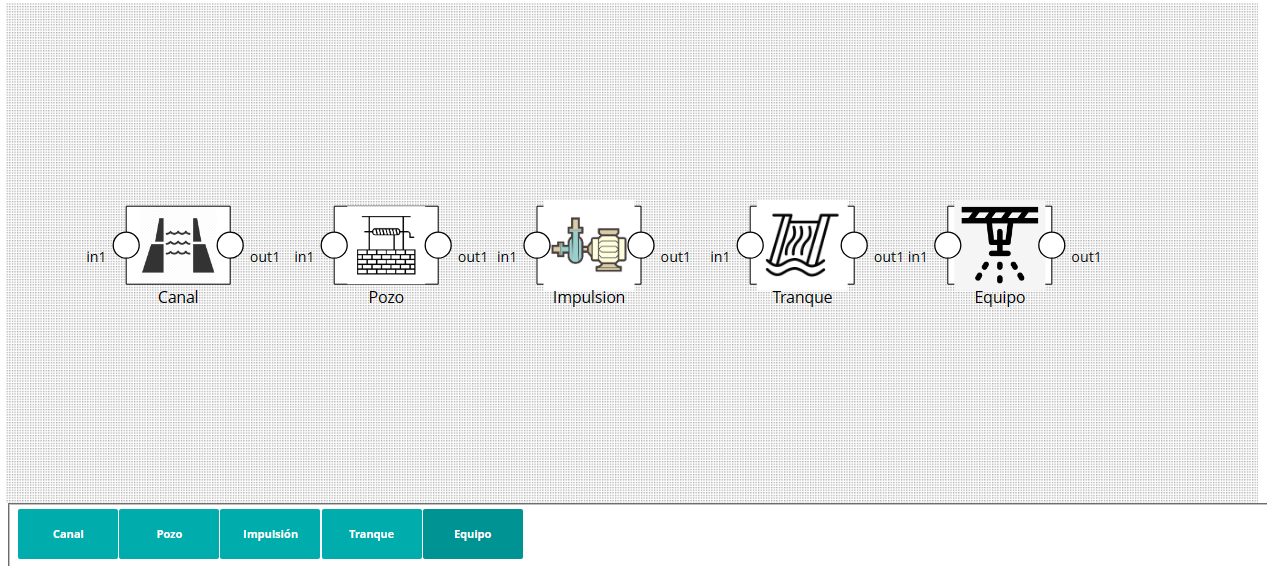
\includegraphics[width=0.8\textwidth]{water-nodes-board}
	\caption{\label{fig:water-nodes-board} Elementos del diagrama. Fuente: Elaboración propia.}
\end{figure}

Las restricciones de conexión se muestran en la figura \ref{fig:water-connections}.

\begin{figure}[H]
	\centering
	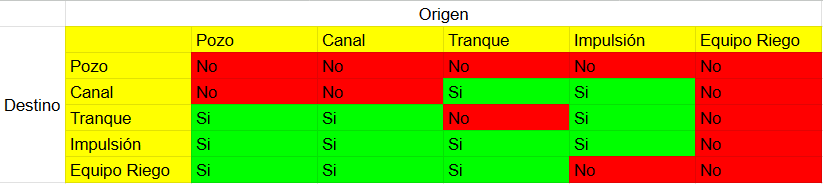
\includegraphics[width=0.8\textwidth]{water-connections}
	\caption{\label{fig:water-connections} Restricciones de conexiones. Fuente: Elaboración propia.}
\end{figure}

Si bien se permite conexiones entre metrahidráulicas del mismo tipo, no se puede hacer una conexión a si mismo.

La conexión entre metahidráulica se conoce como 'Conexiones Metrahidráulicas'. Esta conexión es la flecha que se muestra en la figura \ref{fig:water-conexion-mh}.

\begin{figure}[H]
	\centering
	\includegraphics[width=0.8\textwidth]{water-conexion-mh}
	\caption{\label{fig:water-conexion-mh} Conexión Metrahidráulica. Fuente: Elaboración propia.}
\end{figure}

Cuando una conexión es válida, al arrastrar la flecha desde el \textit{output} de una metahidráulica hacia otra, la flecha se pegará al \textit{input} de la metahidráulica y resaltará (figura \ref{fig:water-valid-connection}). Caso contrario, cuando se arrastra la flecha hacia el \textit{input} de una metahidráulica y esta no se pega, indica que es una conexión no válida (figura \ref{fig:water-invalid-connection}).

\begin{figure}[H]
	\centering
	\includegraphics[width=0.8\textwidth]{water-valid-connection}
	\caption{\label{fig:water-valid-connection} Conexión Metrahidráulica válida. Fuente: Elaboración propia.}
\end{figure}

\begin{figure}[H]
	\centering
	\includegraphics[width=0.8\textwidth]{water-invalid-connection}
	\caption{\label{fig:water-invalid-connection} Conexión Metrahidráulica no válida. Fuente: Elaboración propia.}
\end{figure}

Además de hacer el diagrama, las metrahidráulicas tiene sus propias propiedades, las cuales se pueden asignar haciendo click derecho sobre estas. Al hacer click se abre un formulario al lado de la pizarra con las propiedades de la metrahidráulica escogida.
Los formularios de cada elemento son:
\begin{itemize}
    \item Canal (figura \ref{fig:water-canal-form})
    \item Equipo (figura \ref{fig:water-canal-form})
    \item Impulsión (figura \ref{fig:water-impulsion-form})
    \item Tranque (figura \ref{fig:water-tranque-form})
    \item Pozo (figura \ref{fig:water-pozo-form})
\end{itemize}

\begin{figure}[H]
	\centering
	\includegraphics[width=1\textwidth]{water-canal-form}
	\caption{\label{fig:water-canal-form} Formulario Canal. Fuente: Elaboración propia.}
\end{figure}

\begin{figure}[H]
	\centering
	\includegraphics[width=1\textwidth]{water-equipo-form}
	\caption{\label{fig:water-Equipo-form} Formulario Equipo. Fuente: Elaboración propia.}
\end{figure}

\begin{figure}[H]
	\centering
	\includegraphics[width=1\textwidth]{water-impulsion-form}
	\caption{\label{fig:water-impulsion-form} Formulario Impulsión. Fuente: Elaboración propia.}
\end{figure}

\begin{figure}[H]
	\centering
	\includegraphics[width=1\textwidth]{water-tranque-form}
	\caption{\label{fig:water-tranque-form} Formulario Tranque. Fuente: Elaboración propia.}
\end{figure}

\begin{figure}[H]
	\centering
	\includegraphics[width=1\textwidth]{water-pozo-form}
	\caption{\label{fig:water-pozo-form} Formulario Pozo. Fuente: Elaboración propia.}
\end{figure}

Existen 2 propiedades que están en todos los formularios, los campos de \textit{Inports} y \textit{Outports}. Esta propiedad indica el número de entradas y salidas de la fuente (figura \ref{fig:water-node-ports}).

\begin{figure}[H]
	\centering
	\includegraphics[width=1\textwidth]{water-node-ports}
	\caption{\label{fig:water-node-ports} Entradas y salidas de una fuente. Fuente: Elaboración propia.}
\end{figure}

También, las entradas y salidas tienen propiedades al igual que las metrahidráulicas. Haciendo click derecho sobre las entradas/salidas que estén conectadas, aparece un formulario para asignar las propiedades de la entrada/salida de la metahidráulica (figura \ref{fig:water-conexion-form}).

\begin{figure}[H]
	\centering
	\includegraphics[width=1\textwidth]{water-connection-form}
	\caption{\label{fig:water-conexion-form} Formulario Entrada/Salida. Fuente: Elaboración propia.}
\end{figure}

Para poder eliminar, ya sea una fuente o conexión, se debe pasar el cursor por sobre el elemento para que aparezca un ícono como se muestran en las figuras \ref{fig:water-delete} y \ref{fig:water-delete-connection}.

\begin{figure}[H]
	\centering
	\includegraphics[width=0.8\textwidth]{water-delete}
	\caption{\label{fig:water-delete} Eliminación Fuente. Fuente: Elaboración propia.}
\end{figure}

\begin{figure}[H]
	\centering
	\includegraphics[width=0.8\textwidth]{water-delete-connection}
	\caption{\label{fig:water-delete-connection} Eliminación Conexión Metrahidráulica. Fuente: Elaboración propia.}
\end{figure}

Cuando una entrada/salida tiene un caudalímetro o un sensor de volumen acumulado asignado, este tiene un color rojo, como muestra en la figura \ref{fig:water-port-caudal}.

\begin{figure}[H]
	\centering
	\includegraphics[width=0.8\textwidth]{water-port-caudal}
	\caption{\label{fig:water-port-caudal} Asignación caudalimetro en entrada. Fuente: Elaboración propia.}
\end{figure}

Para poder realizar este diagrama, se utiliza la biblioteca de \textit{JavaScript}, \textit{JointJS}\footnote{\href{https://www.jointjs.com/}{JointJS}}. 
Esta biblioteca permite la creación de diagramas mediante objetos \textit{JSON}, esto ayuda a poder crear y cargar diagramas de una forma más sencilla. Además, esta biblioteca soporta atributos \textit{custom}, lo que permite guardar los datos de los formularios en los \textit{json} de los elementos.
Otro beneficio de esta librería, es la facilidad del trabajo con las entradas y salidas de las fuentes (\textit{ports}\footnote{\href{https://resources.jointjs.com/tutorial/ports}{JointJS: Working with Ports}}) para poder agregar/eliminar \textit{ports}, asignar las propiedades del formulario, entre otras.

Al guardar los cambios se entra a otra configuración para asignar las coordenadas de las metrahidráulicas.
En esta configuración se tiene un mapa junto a una tabla de las fuentes de agua (figura \ref{fig:water-map-view}). La tabla tiene las siguientes columnas:
\begin{enumerate}
    \item Fuente de agua.
    \item Coordenadas.
    \item Acciones (figura \ref{fig:water-table-actions}):
          \begin{itemize}
            \item Editar.
            \item Crear
            \item Eliminar coordenada.
            \item Centrar en mapa.
          \end{itemize}
\end{enumerate}

\begin{figure}[H]
	\centering
	\includegraphics[width=1\textwidth]{water-map-view}
	\caption{\label{fig:water-map-view} Configuración de Coordenadas. Fuente: Elaboración propia.}
\end{figure}

\begin{figure}[H]
	\centering
	\includegraphics[width=0.8\textwidth]{water-table-actions}
	\caption{\label{fig:water-table-actions} Configuración de Coordenadas: Acciones. Fuente: Elaboración propia.}
\end{figure}

Para ingresar las coordenadas de cada fuente, se pueden hacer de dos formas:
\begin{itemize}
    \item Al hacer click en la acción de editar, la fila permitirá editar el nombre de la fuente e ingresar las coordenadas de forma manual, vease figura \ref{fig:water-map-edit}.    
    \item Al hacer click en la acción crear, se mostrará un tooltip que indica que se tiene que hacer click en un lugar del mapa. Al seleccionar el lugar en el mapa se agregará un punto en el mapa y se asignarán las coordenadas a la fuente (figura \ref{fig:water-map-create}).
\end{itemize}

 \begin{figure}[H]
	\centering
	\includegraphics[width=1\textwidth]{water-map-edit}
	\caption{\label{fig:water-map-edit} Acción editar. Fuente: Elaboración propia.}
\end{figure}

\begin{figure}[H]
   \centering
   \includegraphics[width=1\textwidth]{water-map-create}
   \caption{\label{fig:water-map-create} Acción crear. Fuente: Elaboración propia.}
\end{figure}

Al tener las coordenadas asignadas a cada fuente, hacer click en siguiente para guardar.
\fi


\subsection{ENTORNO DE TRABAJO}

\subsubsection{STACK DE TECNOLOGÍAS}

Para el desarrollo en las distintas aplicaciones se tienen los siguientes \textit{stack} de tecnologías:

\begin{itemize}
    \item \textbf{\textit{Admin} de \textit{DropControl}}
    \begin{itemize}
        \item Framework: \textit{React.js}
        \item Componentes: 
        \item IDE: VS Code
        \item Base de Datos: \textit{PostgreSQL}
        \item Hosting: \textit{AWS Amplify}
    \end{itemize}
    \item \textbf{\textit{Operations}}
    \begin{itemize}
        \item Framework: JavaServer Faces
        \item Componentes: Primefaces
        \item IDE: Eclipse
        \item Base de Datos: \textit{MySQL}
        \item Hosting: \textit{AWS EC2}
    \end{itemize}
    \item \textbf{\textit{DropControl}}
    \begin{itemize}
        \item Framework: \textit{React.js}
        \item Componentes: MUI
        \item IDE: VS Code
        \item Base de Datos: \textit{PostgreSQL}
        \item Hosting: \textit{AWS EC2}
    \end{itemize}
    \iffalse\item \textbf{\textit{SETUP}}
    \begin{itemize}
        \item Framework: JavaServer Faces, Primefaces
        \item IDE: Eclipse
        \item Base de Datos: \textit{PostgreSQL}
        \item Hosting: \textit{AWS EC2}
    \end{itemize}\fi
\end{itemize}

\iffalse
Los servicios de WiseConn corren en la nube de \textit{Amazon Web Services}, utilizando los distintos servicios que este ofrece para las bases de datos, \textit{backend} y \textit{hosting}. En las siguientes secciones se explicará el entorno de trabajo de cada aplicación.

\subsubsection{OPERATIONS}

\textit{Operations} es una aplicación interna usada por el área de producción de WiseConn para la gestión de inventario, lotes y despachos.

Es una aplicación monolítica, por lo que, el \textit{backend} y \textit{frontend} se desarrollan juntos en el mismo código. La aplicación está desarrollada en JAVA con \textit{JavaServer Faces}, utilizando el \textit{framework} de \textit{PrimeFaces} y se conecta a una base de datos \textit{MySQL}. \textit{Operations} corre en una instancia \textit{EC2}, mientras que, la base de datos .\

\subsubsection{SETUP}

\textit{SETUP} es una aplicación interna para la configuración de cuentas, campos, sectores, usuarios, entre otros. Utilizado principalmente por el área de soporte de WiseConn.

Es una aplicación monolítica desarrollada en JAVA con \textit{JavaServer Faces}, utilizando el \textit{framework} de \textit{PrimeFaces} y se conecta a la base de datos \textit{PostgreSQL} de \textit{DropControl}.

\subsubsection{ADMIN DE DROPCONTROL}

La aplicación de \textit{Admin} es utilizada por los usuarios administradores de campo para la configuración de campos, sectores, red de nodos, etc.

\textit{Admin} es una aplicación destribuida, es decir, el \textit{backend} y \textit{frontend} están separadas.

Para desplegar la aplicación se utiliza el servicio de \textit{AWS Amplify}, este servicio se encarga de crear/actualizar los recursos del \textit{backend} y de desplegar la aplicación web.

Para el \textit{frontend} se utiliza el framework de \textit{JavaScript}, \textit{React.js}. Además, se utilizan componentes de \textit{Syncfusion}\footnote{\href{https://www.syncfusion.com/react-components}{Syncfusion React Components}}.

Respecto al \textit{backend}, este es \textit{serverless}. Se utilizan funciones \textit{Lambda} con el lenguaje de \textit{JavaScript} que se conectan a una base de datos \textit{PostgreSQL}.
\fi